\documentclass[12pt]{fphw}

\usepackage[utf8]{inputenc}
\usepackage[T1]{fontenc}
\usepackage{mathpazo}
\usepackage{alphabeta}
\usepackage{graphicx}
\usepackage{booktabs}
\usepackage{listings}
\usepackage{enumerate}
\usepackage{hyperref}
\usepackage{amsmath}
\usepackage{framed}
\usepackage[framed]{ntheorem}
\usepackage{amssymb}
\usepackage{xcolor}
\usepackage{tabularx}
\usepackage{tikz}
\usepackage{float}
\usepackage{array}

\graphicspath{{./figures/}}

\setlength{\parskip}{\baselineskip}

\newframedtheorem{frm-thm}{Theorem}
\hypersetup{
    colorlinks=true,
    linkcolor=blue,
    filecolor=magenta,
    urlcolor=cyan,
}
\urlstyle{same}

\title{Deep Learning for NLP -- Homework 2 \\ Response Clarity Classification (CLARITY)}
\author{Αλέξανδρος Γκιάφης \\ ID: sdi2200284}
\date{Spring Semester 2025-2026}
\institute{National and Kapodistrian University of Athens \\ Department of Informatics and Telecommunications}
\class{Artificial Intelligence II (YS19 Μ226 Μ262 Μ325 Μ405)}

\begin{document}
\maketitle

{
  \hypersetup{linkcolor=black}
  \tableofcontents
}
\newpage

\section{Abstract}

Σε αυτή την εργασία είχαμε να φτιάξουμε ένα μοντέλο που, για ένα ζευγάρι ερώτηση--απάντηση από συνέντευξη πολιτικού, αποφασίζει αν η απάντηση είναι \emph{Clear Reply} (όντως απαντάει), \emph{Clear Non-Reply} (αλλάζει εντελώς θέμα) ή \emph{Ambivalent} (κάτι ενδιάμεσο, λέει κάτι αλλά την ίδια στιγμή ξεγλιστράει). Στην πρώτη εργασία είχα κάνει αυτό το πράγμα με κλασικές μεθόδους του τύπου TF-IDF συν Logistic Regression. Εδώ ζητούσαν deep learning -- συγκεκριμένα fine-tuning σε pretrained Transformer μοντέλα.

Δούλεψα και με τα τρία απαιτούμενα μοντέλα (DistilBERT \cite{sanh2019distilbert}, BERT \cite{devlin2019bert}, DeBERTa-v3-base \cite{he2021deberta}). Ξεκίνησα από το πιο μικρό για να μπορέσω να κάνω γρήγορα δοκιμές, και κατέληξα στο DeBERTa σαν το πιο δυνατό. Πάνω από το standard fine-tuning δοκίμασα ένα σωρό πράγματα -- κάποια δούλεψαν, αρκετά όχι, και νομίζω ότι από αυτά που \emph{δεν} δούλεψαν έμαθα περισσότερα.

Το final score στο Kaggle public leaderboard ήταν \textbf{0.69 macro-F1, 31η θέση}. Στο τοπικό μου validation το καλύτερο ensemble έφτασε \textbf{0.7136 macro-F1}. Η διαφορά τοπικού-Kaggle είναι λογική γιατί το test split του Kaggle δεν είναι ακριβώς η ίδια κατανομή με το δικό μου val.

Στις επόμενες ~30 σελίδες θα προσπαθήσω να εξηγήσω όλα τα βήματα μου, τι δοκίμασα, γιατί το δοκίμασα, τι έκανε νόημα και τι όχι. Έχω κάνει συνειδητή προσπάθεια να εξηγώ και τα βασικά (τι είναι ένα Transformer, τι είναι το fine-tuning κ.λπ.) χωρίς να τα θεωρώ self-evident, γιατί όταν εγώ ο ίδιος ξεκίνησα την εργασία δεν τα ήξερα όλα και θα ήθελα να τα είχα διαβάσει κάπου με αυτή τη λογική.

\section{Εισαγωγή -- τι μου ζήτησαν να κάνω}

\subsection{Το CLARITY task σε δύο λόγια}

Το dataset λέγεται CLARITY. Είναι μια συλλογή από ζευγάρια ερώτηση--απάντηση που έχουν παρθεί από συνεντεύξεις και press conferences πολιτικών (κυρίως αμερικανών προέδρων -- Bush, Obama κ.λπ.). Η δουλειά μου ήταν, για κάθε τέτοιο ζευγάρι, να φτιάξω ένα μοντέλο που να βγάζει ένα από τρία labels:

\begin{itemize}
    \item \textbf{Clear Reply} -- ο πολιτικός όντως απαντάει στην ερώτηση. Πχ:
    \begin{quote}
    \emph{Q: What more can be done to prevent that from happening?} \\
    \emph{A: We've put a lot into ethanol. And we're working on cellulosic ethanol \dots}
    \end{quote}
    Δηλαδή λέει συγκεκριμένα τι κάνουν.

    \item \textbf{Clear Non-Reply} -- ο πολιτικός ξεφεύγει εντελώς. Δεν απαντάει. Μπορεί να λέει ``I won't talk about that'', μπορεί να αλλάζει θέμα, μπορεί να σχολιάζει την ερώτηση αλλά χωρίς να δίνει απάντηση. Πχ:
    \begin{quote}
    \emph{Q: Specifically, have you seen any success in your diplomatic strategy so far?} \\
    \emph{A: Well, I think you know me well enough to know that I don't like talking about whether I see success or not\dots}
    \end{quote}

    \item \textbf{Ambivalent} -- η μεγάλη ``γκρίζα ζώνη''. Ο πολιτικός λέει \emph{κάτι} σχετικό αλλά την ίδια στιγμή υπεκφεύγει, μιλάει γενικόλογα, ή απαντάει σε μέρος της ερώτησης αλλά όχι όλη. Στατιστικά αυτή η κατηγορία είναι περίπου το 60\% του dataset, οπότε από μόνη της δημιουργεί τεράστιο class imbalance.
\end{itemize}

Το πρόβλημα δεν είναι απλό. Δεν αρκεί να μετρήσω αν η απάντηση περιέχει λέξεις της ερώτησης (αυτό σπάνια κρίνει τη clarity). Πρέπει να ``καταλάβει'' το μοντέλο τη \emph{στάση} της απάντησης απέναντι στην ερώτηση -- κάτι που γλωσσικά λέγεται discourse-level reasoning. Είναι αρκετά subtle πράγμα.

\subsection{Τι ζητάει συγκεκριμένα η εκφώνηση του Homework 2}

Πέρα από το γενικό task, το assignment βάζει συγκεκριμένους περιορισμούς:

\begin{enumerate}
    \item Να γίνει fine-tuning τριών συγκεκριμένων pretrained Transformer μοντέλων: \texttt{bert-base-uncased}, \texttt{distilbert-base-uncased}, και \texttt{microsoft/deberta-v3-base}.
    \item Να χρησιμοποιήσω PyTorch και Hugging Face Transformers library.
    \item Να γράψω εγώ το explicit training loop -- \emph{απαγορεύεται} το Hugging Face \texttt{Trainer} API. (Ως δικαιολογία για τον κανόνα: είναι εκπαιδευτικό να ξέρεις τι κάνει το Trainer εσωτερικά.)
    \item Να αποφασίσω μόνος μου τα πάντα: input format, hyperparameters, validation strategy, regularization, αν θα χειριστώ class imbalance, κ.λπ.
    \item Να παραδώσω \emph{τρία} ξεχωριστά Kaggle notebooks (ένα ανά μοντέλο) και \emph{ένα} report (αυτό).
    \item Στο report να συμπεριλάβω: hyperparameter analysis, input formulation analysis, model comparison με βάση accuracy / precision / recall / F1 / macro-F1, subgroup analysis (πχ ανά μήκος ερώτησης/απάντησης), error analysis με συγκεκριμένα παραδείγματα, και discussion των modifications που δοκίμασα.
\end{enumerate}

\subsection{Η αρχική μου σύγχυση}

Δεν θα κρύψω ότι όταν πρωτοδιάβασα την εκφώνηση είχα μια στιγμή πανικού. Είχα ξανακούσει για BERT αλλά δεν ήξερα τι ήταν το DistilBERT ή το DeBERTa. Δεν είχα ποτέ γράψει custom training loop σε PyTorch -- είχα κάνει training loops αλλά πάντα στο Trainer API ή σε άλλα frameworks. Δεν ήξερα τι σημαίνει ``fine-tuning'' στην πράξη.

Πέρασα τις πρώτες ώρες να διαβάζω. Διάβασα τα course slides (\emph{Transformers}, \emph{BERT}), έπιασα και ένα τμήμα του Hugging Face course στο Internet, και ξανακοίταξα τα δικά μου από την HW1. Σιγά σιγά συνειδητοποίησα τι ζητάει η εργασία. Επειδή ήδη έχω επενδύσει χρόνο σε αυτή την επανατοποθέτηση, σκέφτηκα ότι αξίζει να το βάλω στο ίδιο το report -- να εξηγήσω και εγώ τα βασικά για όποιον τα διαβάζει χωρίς να τα ξέρει. Είναι το επόμενο section.

\section{Πριν προχωρήσω -- βασικές έννοιες για όποιον δεν τις ξέρει}

Σε αυτό το section θα κάνω μια προσπάθεια να εξηγήσω τα concepts που χρησιμοποιώ μετά. Δεν είναι θεωρητικά σχολαστικό -- ο σκοπός είναι ένας αναγνώστης που δεν ξέρει τι είναι ένα Transformer ή ένα cross-entropy loss να μπορεί να καταλάβει το report. Αν τα ξέρετε όλα, μπορείτε να προσπεράσετε.

\subsection{Τι είναι ένα νευρωνικό δίκτυο}

Με την πιο απλή εξήγηση: ένα νευρωνικό δίκτυο είναι μια \emph{μαθηματική συνάρτηση} με πολλές παραμέτρους (που τις λέμε ``βάρη'' ή ``weights''), η οποία παίρνει input έναν αριθμό ή ένα διάνυσμα αριθμών και βγάζει output έναν άλλο αριθμό ή διάνυσμα. Το ``νευρωνικό'' στο όνομα είναι ιστορικό -- λέγεται έτσι επειδή στις απαρχές του (δεκαετίες πίσω) το έφτιαξαν ώστε να μοιάζει με την ιδέα του πώς δουλεύουν τα νευρώνια στον εγκέφαλο. Στην πραγματικότητα είναι απλώς πολλαπλασιασμοί πινάκων ακολουθούμενοι από μη-γραμμικές συναρτήσεις (πχ ReLU: $f(x) = \max(0, x)$).

Φαντάσου ένα δίκτυο σαν ένα μηχάνημα με πάρα πολλά κουμπιά (τα weights). Όταν του δίνεις input, αυτά τα κουμπιά πολλαπλασιάζουν, προσθέτουν, και βγάζουν ένα output. Το ``learning'' είναι η διαδικασία να ρυθμίσουμε τα κουμπιά έτσι ώστε για τα δεδομένα μας να βγάζει σωστές προβλέψεις.

Το πρόβλημα είναι ότι τα weights είναι εκατομμύρια. Δεν μπορούμε να τα ρυθμίσουμε με το χέρι. Γι' αυτό υπάρχει το gradient descent.

\subsection{Gradient descent με απλά λόγια}

Φαντάσου ότι στέκεσαι σε έναν λόφο με κλειστά μάτια και θέλεις να φτάσεις στο πιο βαθύ σημείο της κοιλάδας. Δεν βλέπεις τίποτα. Αυτό που μπορείς να κάνεις είναι να αισθανθείς με τα πόδια σου ποια κατεύθυνση κατεβαίνει πιο απότομα, και να κάνεις ένα μικρό βήμα προς εκείνη την κατεύθυνση. Μετά από πολλά τέτοια βήματα, θα φτάσεις σε κάποιο βαθύ σημείο.

Αυτό ακριβώς είναι το gradient descent. Έχουμε μια συνάρτηση -- το \emph{loss} -- που μας λέει πόσο ``λάθος'' είναι το μοντέλο μας πάνω στα δεδομένα μας (όσο πιο μικρό loss, τόσο καλύτερα προβλέπει). Το gradient (η ``κλίση'') μας λέει σε ποια κατεύθυνση πρέπει να αλλάξουμε τα weights για να μειωθεί το loss. Παίρνουμε ένα μικρό βήμα προς εκείνη την κατεύθυνση. Επαναλαμβάνουμε.

Το μέγεθος του βήματος ονομάζεται \emph{learning rate}. Αν είναι πολύ μεγάλο, μπορεί να ``υπερπηδήσουμε'' την κοιλάδα και να βρεθούμε στην απέναντι πλαγιά. Αν είναι πολύ μικρό, χρειάζεται αιωνιότητα να φτάσουμε. Συνήθως δοκιμάζουμε διάφορες τιμές (στη δουλειά μου εδώ δοκίμασα 1e-5, 2e-5, 3e-5, 5e-5).

Το ``ποια κατεύθυνση κατεβαίνει'' το υπολογίζουμε με backpropagation, που είναι ουσιαστικά ο κανόνας της αλυσίδας από τον απειροστικό λογισμό εφαρμοσμένος σε όλο το δίκτυο. Αυτό το κάνει αυτόματα η PyTorch, οπότε δεν θα μπω σε λεπτομέρειες.

Ο αλγόριθμος που υλοποιεί τα βήματα ονομάζεται \emph{optimizer}. Στη δουλειά μου χρησιμοποιώ AdamW, που είναι μια εκλεπτυσμένη εκδοχή του gradient descent με δυο επιπλέον tricks: κρατάει momentum (κατευθύνεται όχι μόνο από τη στιγμή αλλά και από προηγούμενα βήματα) και προσαρμόζει το learning rate ξεχωριστά για κάθε weight (adaptive learning rate). Πιο κάτω εξηγώ καλύτερα τι κάνει.

\subsection{Loss functions: πώς μετράμε ``πόσο λάθος είμαστε''}

Για classification problem, η συνηθισμένη loss είναι το \emph{cross-entropy}. Μην τρομάζετε από το όνομα -- η ιδέα είναι απλή.

Έστω ότι έχουμε 3 κλάσεις (CR, AMB, CNR). Το μοντέλο μας βγάζει \emph{logits} -- 3 αριθμούς που ``δείχνουν'' πόσο πιστεύει ότι το input ανήκει σε κάθε κλάση. Πχ μπορεί να βγάλει $[1.5, 2.3, -0.4]$. Αυτοί οι αριθμοί δεν είναι πιθανότητες (δεν αθροίζουν 1, και μπορούν να είναι αρνητικοί). Για να τους κάνουμε πιθανότητες, εφαρμόζουμε \emph{softmax}:
\[
p_i = \frac{e^{z_i}}{\sum_j e^{z_j}}
\]
Αυτό μας δίνει $[0.27, 0.61, 0.12]$ -- τώρα αθροίζουν 1 και μπορούμε να τα διαβάσουμε ως ``το μοντέλο πιστεύει 27\% CR, 61\% AMB, 12\% CNR''.

Το cross-entropy loss είναι:
\[
L = -\log(p_{\text{σωστή κλάση}})
\]
Δηλαδή αν η σωστή κλάση είναι AMB και το μοντέλο έδωσε 0.61 πιθανότητα στο AMB, το loss είναι $-\log(0.61) \approx 0.49$. Αν το μοντέλο είχε δώσει 0.99 στο AMB, το loss θα ήταν $-\log(0.99) \approx 0.01$, πολύ μικρότερο. Αν είχε δώσει 0.01 στο AMB (τραγικά λάθος), το loss θα ήταν $-\log(0.01) \approx 4.6$, τεράστιο.

Κάθε batch έχει πολλά παραδείγματα -- παίρνουμε τη μέση τιμή του cross-entropy πάνω σε όλα.

\subsection{Λίγα λόγια για embeddings (πώς γίνονται οι λέξεις αριθμοί)}

Ένας υπολογιστής δεν καταλαβαίνει ``λέξεις'' -- καταλαβαίνει αριθμούς. Πώς λοιπόν μπορεί ένα νευρωνικό δίκτυο να επεξεργαστεί κείμενο;

Η απάντηση είναι: μετατρέπουμε κάθε λέξη σε ένα διάνυσμα αριθμών. Αυτό λέγεται \emph{embedding}. Πχ η λέξη ``cat'' μπορεί να γίνει το διάνυσμα $[0.21, -0.43, 0.10, \dots, 0.66]$ με 768 διαστάσεις (στο BERT).

Τα embeddings μαθαίνονται κατά το pretraining έτσι ώστε λέξεις με παρόμοιο νόημα να βρίσκονται κοντά στον χώρο. Η κλασική δοκιμή είναι το ``king minus man plus woman approximately equals queen'' -- δείχνει ότι τα embeddings έχουν συγκρατήσει σημασιολογικές σχέσεις.

Στα σύγχρονα Transformer μοντέλα, η αναπαράσταση κάθε λέξης δεν είναι σταθερή. Είναι \emph{contextual} -- αλλάζει ανάλογα με τις γύρω λέξεις. Πχ το ``bank'' στο ``river bank'' και στο ``bank account'' βγάζει διαφορετικά διανύσματα, γιατί η self-attention (που εξηγώ πιο κάτω) ``βλέπει'' τα γειτονικά tokens.

\subsection{Pretraining και fine-tuning}

Αυτό είναι ίσως το πιο σημαντικό concept για να καταλάβει κανείς γιατί δουλεύουν τα Transformer μοντέλα.

\textbf{Pretraining}: παίρνουμε ένα τεράστιο dataset (πχ όλη τη Wikipedia, books, τμήμα του internet -- κάποια εκατομμύρια ή δισεκατομμύρια λέξεις) και εκπαιδεύουμε το μοντέλο πάνω σε ένα γενικό task. Στο BERT, αυτό το task είναι ``masked language modeling'': παίρνουμε μια πρόταση, σβήνουμε τυχαία 15\% των λέξεων, και ζητάμε από το μοντέλο να μαντέψει ποιες ήταν. Πχ αν δώσουμε ``The cat sat on the [MASK]'', το μοντέλο πρέπει να καταλάβει ότι η σβησμένη λέξη είναι μάλλον ``mat'' ή ``floor''.

Με αυτή την εκπαίδευση, το μοντέλο μαθαίνει γενικά γλωσσικά patterns: σύνταξη, σημασιολογία, παραφράσεις, common sense, ακόμα και λίγη γνώση για τον κόσμο. Αυτή η εκπαίδευση είναι ακριβή -- κοστίζει εκατοντάδες χιλιάδες δολάρια σε GPUs -- αλλά γίνεται μία φορά και τα weights δημοσιεύονται. Έτσι εμείς απλώς τα κατεβάζουμε.

\textbf{Fine-tuning}: παίρνουμε αυτό το pretrained μοντέλο, βάζουμε από πάνω ένα μικρό classifier (στην περίπτωσή μας: ένα linear layer που βγάζει 3 logits, ένα ανά κλάση), και \emph{συνεχίζουμε} την εκπαίδευση πάνω στο δικό μας πιο μικρό dataset. Δηλαδή τα weights που είχαν μάθει γενικά γλωσσικά patterns προσαρμόζονται λίγο για να είναι καλά στο specific task μας (clarity classification).

Γιατί δουλεύει αυτό; Γιατί η γενική γλωσσική γνώση είναι transferable. Δεν χρειάζεται να μάθουμε από το μηδέν τι σημαίνει ``hedge'' ή ``deflection'' -- το μοντέλο τα ξέρει ήδη.

\subsection{Backbone vs head}

Όταν λέμε ``backbone'' εννοούμε το pretrained τμήμα του δικτύου -- το BERT/DistilBERT/DeBERTa κομμάτι. Είναι σαν τη ραχοκοκαλιά του μοντέλου, που έχει ήδη μάθει τη γλώσσα.

Όταν λέμε ``head'' (ή ``classification head'') εννοούμε το νέο, μικρό κομμάτι που βάλαμε από πάνω για το συγκεκριμένο task. Συνήθως είναι 1-2 linear layers που μετατρέπουν την αναπαράσταση του backbone σε logits.

Το head ξεκινάει με τυχαίες παραμέτρους και πρέπει να μάθει από το μηδέν. Το backbone ξεκινάει με τα pretrained weights και απλώς προσαρμόζεται. Γι' αυτό συνήθως δίνουμε στο head μεγαλύτερο learning rate (μου το έμαθε με τον δύσκολο τρόπο, δες παρακάτω για το DeBERTa).

\subsection{Tokenization -- πώς σπάμε τις λέξεις}

Ο tokenizer μετατρέπει το ωμό κείμενο σε λίστα από integer IDs που ταΐζουμε στο μοντέλο. Δεν δουλεύει σε επίπεδο λέξης -- δουλεύει σε επίπεδο \emph{subword}, χρησιμοποιώντας έναν αλγόριθμο όπως WordPiece (BERT) ή SentencePiece (DeBERTa).

Παράδειγμα: η λέξη ``unhappiness'' δεν υπάρχει στο vocabulary. Ο WordPiece tokenizer τη σπάει σε [``un'', ``happi'', ``\#\#ness''] (τα ``\#\#'' υποδηλώνουν ότι το token είναι συνέχεια προηγούμενου, όχι αρχή λέξης). Με αυτόν τον τρόπο, ακόμα και αν δεν έχει ξαναδεί τη συγκεκριμένη λέξη, μπορεί να την αναπαραστήσει από τα γνωστά κομμάτια.

Αυτό είναι σημαντικό για το συγκεκριμένο dataset, γιατί οι πολιτικοί χρησιμοποιούν ονόματα ανθρώπων, ονόματα τόπων, και specific terms που μπορεί να μην υπάρχουν στο vocabulary. Με subword tokenization δεν χάνονται.

Ένα ακόμα πράγμα: κάθε input ξεκινάει με ένα ειδικό token \texttt{[CLS]}. Μετά το pass από το μοντέλο, το embedding που αντιστοιχεί στο \texttt{[CLS]} τοποθετείται έτσι ώστε να ``περιέχει'' περιεκτικά πληροφορία για όλη την πρόταση. Πάνω σε αυτό βάζουμε τον classifier head για να βγάλουμε labels. (Αυτό λέγεται και ``pooled output''.)

\subsection{Self-attention σε δύο παραγράφους}

Self-attention είναι ο πυρήνας του Transformer. Η ιδέα: για να φτιάξουμε την αναπαράσταση μιας λέξης, αντί να χρησιμοποιήσουμε μόνο τη γειτονιά της (όπως στα RNN ή τα CNN), αφήνουμε κάθε λέξη να ``κοιτάξει'' \emph{όλες} τις άλλες λέξεις στην πρόταση και να αποφασίσει ποιες είναι σχετικές.

Συγκεκριμένα: για κάθε token, υπολογίζουμε ένα ``query'' vector, ένα ``key'' vector, και ένα ``value'' vector (γραμμικοί μετασχηματισμοί). Το score attention μεταξύ token A και token B είναι το dot product του query του A με το key του B (αν είναι μεγάλο, σημαίνει ``το A βλέπει το B σαν σημαντικό''). Κανονικοποιούμε με softmax πάνω σε όλα τα Β. Η νέα αναπαράσταση του A είναι το weighted average των values όλων των B's με βάση αυτά τα scores.

Με απλά λόγια: ``για κάθε λέξη, ποιες άλλες λέξεις της πρότασης είναι ενδιαφέρουσες, και πάρε weighted average αυτών για να φτιάξεις μια καινούρια αναπαράσταση''. Είναι σαν να επιτρέπεις στις λέξεις να ``μιλήσουν'' μεταξύ τους.

Αυτό γίνεται πολλές φορές στη σειρά (multi-head attention, πολλά layers το ένα πάνω στο άλλο). Ένα Transformer μοντέλο τύπου BERT-base έχει 12 τέτοια layers.

\subsection{Τι είναι λοιπόν ένα Transformer}

Ένα Transformer είναι: stack από layers, όπου κάθε layer είναι (multi-head self-attention) + (feedforward network) + (residual connections + layer norm). Repeat 12 times (BERT-base) ή 6 times (DistilBERT) ή 12 times (DeBERTa-v3-base).

Στο τέλος έχουμε για κάθε token μια αναπαράσταση 768 διαστάσεων (το ``hidden size''). Παίρνουμε την αναπαράσταση του \texttt{[CLS]} token, την περνάμε από έναν classifier (linear layer), και βγαίνουν οι 3 logits για τις 3 κλάσεις.

\subsection{Dropout, layer normalization, regularization}

Τρία concepts που εμφανίζονται μέσα στα Transformer αρχιτεκτονικά αλλά τα χρησιμοποίησα και στον classifier head μου.

\textbf{Dropout}: κατά το training, σε κάθε batch ``σβήνουμε'' τυχαία (πχ) 10\% των νευρώνων (τους θέτουμε στο 0). Αυτό αναγκάζει το μοντέλο να μη βασίζεται σε λίγους συγκεκριμένους νευρώνες -- πρέπει να μάθει redundant representations. Είναι μια μορφή regularization που μειώνει το overfitting (πιο κάτω). Στο inference (testing) δεν εφαρμόζεται dropout.

\textbf{Layer normalization}: κανονικοποιεί τις τιμές των activations μέσα σε κάθε layer ώστε να έχουν μέσο όρο 0 και τυπική απόκλιση 1. Βοηθάει την εκπαίδευση να είναι σταθερότερη -- αλλιώς τα activations μπορούν να ``εκραγούν'' ή να ``εξαφανιστούν'' καθώς περνάνε από layers.

\textbf{Regularization} (γενικά): κάθε τεχνική που εμποδίζει το μοντέλο να ``μαθαίνει απ' έξω'' το training set. Άλλες μορφές: weight decay (penalizing μεγάλα weights), early stopping (σταματάμε όταν το val αρχίσει να χειροτερεύει), data augmentation. Όλα στοχεύουν στο να γενικεύει το μοντέλο σε άγνωστα δεδομένα.

\subsection{Overfitting, validation set, hyperparameters}

\textbf{Overfitting}: το μοντέλο μαθαίνει τόσο καλά το training set που αρχίζει να αποστηθίζει αντί να γενικεύει. Συμπτώματα: το train loss συνεχίζει να πέφτει αλλά το validation loss σταματάει να μειώνεται ή αρχίζει να αυξάνεται. Σαν ένας μαθητής που αποστηθίζει τις απαντήσεις στις ασκήσεις του φυλλαδίου αλλά αποτυγχάνει στο διαγώνισμα όταν πέσουν παραλλαγές.

\textbf{Validation set}: ένα κομμάτι δεδομένων που το \emph{δεν} χρησιμοποιούμε για training. Το χρησιμοποιούμε για να μετράμε πόσο καλά γενικεύει το μοντέλο και να επιλέξουμε hyperparameters. Στη δουλειά μου χρησιμοποίησα 10\% του dataset (342 από 3412) σαν validation. Δεν χρησιμοποίησα cross-validation για λόγους χρόνου και GPU κόστους -- θα το εξηγήσω παρακάτω.

\textbf{Hyperparameters}: παράμετροι που \emph{δεν} μαθαίνει το μοντέλο μέσω gradient descent αλλά τις βάζουμε εμείς. Πχ learning rate, batch size, number of epochs, max sequence length, dropout rate, weight decay. Η επιλογή τους είναι τέχνη -- δοκιμάζεις διαφορετικές τιμές, κρατάς αυτή που έδωσε καλύτερο val score.

\subsection{Mini-glossary για τους υπόλοιπους όρους}

Για να μην κουράζω, λίγοι ακόμα όροι που θα συναντήσετε:

\begin{itemize}
    \item \textbf{Batch}: ένα μικρό σύνολο παραδειγμάτων (πχ 16) που το μοντέλο επεξεργάζεται μαζί σε ένα forward+backward pass. Το loss υπολογίζεται μέσω αυτών των 16, και τα weights ενημερώνονται μία φορά.
    \item \textbf{Epoch}: ένα ολόκληρο πέρασμα πάνω σε όλο το training set. Στη δουλειά μου χρησιμοποίησα συνήθως 3-5 epochs.
    \item \textbf{Step / iteration}: ένα update των weights -- δηλαδή ένα batch.
    \item \textbf{Logits}: οι μη-κανονικοποιημένες τιμές του classifier (πριν το softmax).
    \item \textbf{Probabilities}: μετά το softmax, οι τιμές αθροίζουν 1 και τις διαβάζουμε σαν πιθανότητες.
    \item \textbf{Argmax}: η κλάση με την μεγαλύτερη probability -- αυτή που τελικά προβλέπει το μοντέλο.
    \item \textbf{Seed}: ο αριθμός που αρχικοποιεί τα random number generators. Με ίδιο seed παίρνεις ίδια αποτελέσματα. Στα Transformers, διαφορετικό seed = διαφορετική τυχαία αρχικοποίηση του head + διαφορετικό dropout pattern + διαφορετική σειρά shuffling των batches = αρκετά διαφορετικό τελικό μοντέλο.
    \item \textbf{Inference}: όταν χρησιμοποιούμε ένα εκπαιδευμένο μοντέλο για να βγάλει προβλέψεις (όχι training).
    \item \textbf{Macro-F1}: εξηγώ αναλυτικά παρακάτω, αλλά συνοπτικά: F1 σκορ ξεχωριστά ανά κλάση, μετά μέσος όρος. Αναγκάζει το μοντέλο να είναι καλό σε όλες τις κλάσεις, όχι μόνο στην επικρατούσα.
\end{itemize}

OK, νομίζω αυτά είναι αρκετά για βάσεις. Πάμε στο πραγματικό περιεχόμενο.

\section{Τα τρία μοντέλα -- αναλυτικός οδηγός}

Επειδή η εργασία απαιτεί τη χρήση τριών συγκεκριμένων μοντέλων, πιστεύω ότι αξίζει να εξηγήσω τι είναι το καθένα και γιατί διαφέρουν. Δεν είναι όλα ισοδύναμα, και η επιλογή ενός από αυτά (DeBERTa) ως ``πρωταγωνιστή'' βασίστηκε στην απόδοσή του.

\subsection{BERT (\texttt{bert-base-uncased})}

Το \emph{Bidirectional Encoder Representations from Transformers} -- ή πιο απλά BERT \cite{devlin2019bert} -- είναι το πρώτο πραγματικά επιτυχημένο pretrained Transformer για NLP tasks. Ήρθε από τη Google το 2018 και άλλαξε τα πάντα στο NLP.

\textbf{Αρχιτεκτονική}: 12 layers Transformer encoder, hidden size 768, 12 attention heads, 110M παραμέτρους συνολικά.

\textbf{Pretraining tasks (δηλαδή τι εκπαιδευόταν να κάνει στο τεράστιο corpus πριν δει εμάς)}:
\begin{itemize}
    \item \emph{Masked Language Modeling (MLM)}: σβήνουμε το 15\% των tokens και ζητάμε να τα μαντέψει.
    \item \emph{Next Sentence Prediction (NSP)}: δίνουμε δύο προτάσεις και ρωτάμε αν η δεύτερη είναι όντως η επόμενη της πρώτης ή τυχαία. Αυτό βοηθάει το μοντέλο να μάθει sentence-level σχέσεις.
\end{itemize}

\textbf{Bidirectional}: Σε αντίθεση με τα GPT-style μοντέλα που διαβάζουν left-to-right, στο BERT κάθε token κοιτάει \emph{και} αριστερά \emph{και} δεξιά μέσα στην πρόταση μέσω της self-attention. Αυτό το κάνει πιο δυνατό για understanding tasks (όπως classification), αλλά λιγότερο κατάλληλο για generation tasks.

\textbf{``uncased''}: το \texttt{bert-base-uncased} έχει vocabulary που δεν διακρίνει κεφαλαία/πεζά. Δηλαδή ``Hello'' και ``hello'' γίνονται το ίδιο token. Αυτό χάνει λίγη πληροφορία (πχ proper nouns) αλλά βοηθάει σε γενικά tasks γιατί μειώνει το vocabulary και αυξάνει το data per token.

Στη δουλειά μου, το BERT έδωσε best score 0.6417 macro-F1 στο val set (seed=1). Πολύ κοντά στο DistilBERT, και αρκετά κάτω από το DeBERTa.

\subsection{DistilBERT (\texttt{distilbert-base-uncased})}

Το DistilBERT \cite{sanh2019distilbert} είναι μια μικρότερη και ταχύτερη version του BERT, φτιαγμένη με μια τεχνική που λέγεται \emph{knowledge distillation}.

\subsubsection{Τι είναι το knowledge distillation}

Φαντάσου τη σχέση δασκάλου-μαθητή. Έχουμε ήδη ένα μεγάλο, καλά εκπαιδευμένο μοντέλο (το ``teacher'' -- εδώ BERT). Θέλουμε να φτιάξουμε ένα μικρότερο μοντέλο (το ``student'') που να κάνει σχεδόν τα ίδια.

Η αφελής προσέγγιση: εκπαιδεύουμε το student με ίδιο τρόπο (MLM στο corpus). Αλλά το student είναι πιο μικρό, οπότε χάνει capacity, οπότε και ποιότητα.

Η έξυπνη προσέγγιση (knowledge distillation): εκπαιδεύουμε το student όχι απλά να μαντέψει τα labels (sparse targets), αλλά \emph{να μιμηθεί τις probabilities που βγάζει το teacher} (soft targets). Δηλαδή για κάθε masked token, το teacher βγάζει ένα probability distribution πάνω σε όλο το vocabulary -- και αναγκάζουμε το student να βγάζει παρόμοιο distribution. Αυτό είναι πολύ πιο ``πλούσιο'' σήμα από ένα binary correct/incorrect.

Με αυτή την τεχνική, το DistilBERT καταφέρνει να είναι:
\begin{itemize}
    \item 40\% μικρότερο από το BERT (66M params αντί 110M, 6 layers αντί 12),
    \item 60\% γρηγορότερο,
    \item Διατηρεί το 97\% της απόδοσης του BERT σε γενικά benchmarks.
\end{itemize}

Δηλαδή ένα ``μαθητής'' που έμαθε να μιμείται τον δάσκαλο, και τα κατάφερε σχεδόν εξίσου καλά με λιγότερα κουμπιά.

\subsubsection{Σημαντικές διαφορές vs BERT}

\begin{itemize}
    \item Δεν έχει NSP loss στο pretraining (αφαιρέθηκε επειδή έδειξε ότι δεν βοηθάει πολύ).
    \item \textbf{Δεν έχει token type IDs / segment embeddings}. Αυτό είναι κρίσιμο για το δικό μας task: στο BERT/DeBERTa μπορώ να πω ``αυτά τα tokens είναι η ερώτηση, αυτά είναι η απάντηση'' με token\_type\_ids = 0 ή 1. Στο DistilBERT αυτή η πληροφορία χάνεται -- το μοντέλο βλέπει μόνο μια ενιαία ακολουθία tokens χωρισμένη με \texttt{[SEP]}.
\end{itemize}

Επέλεξα το DistilBERT σαν το πιο μικρό μοντέλο για να κάνω fast iteration στα πειράματα. Αν μια ιδέα δεν δούλευε εδώ, σπάνια άξιζε να σπαταλήσω χρόνο σε BERT/DeBERTa. Στη δουλειά μου το DistilBERT έδωσε best score 0.6405 macro-F1 (seed=42, ml=512, lr=3e-5, 3 epochs).

\subsection{DeBERTa-v3-base (\texttt{microsoft/deberta-v3-base})}

Το DeBERTa \cite{he2021deberta} είναι το ``έξυπνο'' στοιχείο της οικογένειας. Ήρθε από τη Microsoft και κάνει δύο σημαντικά πράγματα διαφορετικά σε σχέση με το BERT:

\subsubsection{Disentangled attention -- η βασική καινοτομία}

Στο BERT, το embedding κάθε token είναι ένα διάνυσμα που περιέχει \emph{και} το ``τι σημαίνει η λέξη'' \emph{και} το ``σε ποια θέση βρίσκεται μέσα στην πρόταση''. Αυτό γίνεται προσθέτοντας στο word embedding ένα positional embedding. Πχ:
\[
\text{embedding}(\text{``cat''}_{\text{position 3}}) = E_{\text{word}}(\text{cat}) + E_{\text{pos}}(3)
\]
Έπειτα η self-attention πολλαπλασιάζει αυτό το αναμεμειγμένο διάνυσμα με weights για να βρει τα query/key/value.

Το DeBERTa λέει: ``στάσου, αυτό είναι sub-optimal. Το \emph{τι} σημαίνει η λέξη και το \emph{πού} βρίσκεται είναι δύο διαφορετικά πράγματα -- ας τα κρατήσουμε ξεχωριστά''.

Έτσι το DeBERTa υπολογίζει την attention ως άθροισμα τριών components:
\begin{itemize}
    \item \emph{content-to-content attention}: πόσο σχετικό είναι το νόημα της λέξης A με το νόημα της λέξης B
    \item \emph{content-to-position attention}: πόσο σχετικό είναι το νόημα της A με τη \emph{σχετική θέση} της B
    \item \emph{position-to-content attention}: πόσο σχετική είναι η θέση της A με το νόημα της B
\end{itemize}

Με αυτή τη ``διαλέξη'' (``disentangled''), το μοντέλο μπορεί να εκφράσει πιο πλούσιες σχέσεις. Πχ μπορεί να μάθει ``η λέξη ‘not' στην ίδια πρόταση είναι σημαντική ανεξαρτήτως θέσης, αλλά πιο σημαντική όταν είναι ακριβώς πριν από verb''.

\subsubsection{Enhanced mask decoder}

Στο pretraining, αντί να προβλέπει την σβησμένη λέξη μόνο από context, το DeBERTa χρησιμοποιεί επιπλέον \emph{absolute positional information} στο τελευταίο layer πριν την πρόβλεψη. Δηλαδή ξέρει εκτός από context, και ακριβώς ποια θέση είναι αυτή που σβήσαμε. Αυτό βοηθάει σε ορισμένες περιπτώσεις (πχ syntactic restoration).

\subsubsection{``v3'': τι αλλάζει στην v3}

Η original έκδοση του DeBERTa εκπαιδεύτηκε με MLM (masked language modeling) όπως το BERT. Η v3 χρησιμοποιεί \emph{replaced token detection} -- το pretraining task από το ELECTRA. Αντί να σβήνουμε λέξεις και να ζητάμε να τις μαντέψει, αντικαθιστούμε τυχαίες λέξεις με ``φευδείς'' λέξεις (που τις βγάζει ένα μικρότερο μοντέλο που λέγεται generator) και ζητάμε από το DeBERTa να βρει ποιες είναι αληθινές και ποιες αντικαταστάθηκαν.

Γιατί αυτό βοηθάει; Γιατί στο MLM το μοντέλο λαμβάνει σήμα μόνο από το 15\% των tokens (αυτά που σβήνουμε). Στο replaced token detection, λαμβάνει σήμα από \emph{όλα} τα tokens (κάθε ένα είναι binary classification: είναι real ή replaced). Αυτό είναι 6-7 φορές πιο sample-efficient.

Συνέπεια: το DeBERTa-v3-base, με ίδια params (~140M), νικάει το BERT-large (340M) σε αρκετά benchmarks. Στη δική μου δουλειά, το DeBERTa-v3-base έδωσε best single 0.6962 (vs 0.6417 του BERT). Αυτό είναι ένα τεράστιο +0.05 για NLP standards.

\subsection{Γιατί επέλεξα το DeBERTa σαν workhorse}

Αφού είδα ότι το DeBERTa έδινε καθαρά καλύτερο val score, αποφάσισα να επικεντρώσω τον υπόλοιπο χρόνο μου σε πειραματισμό \emph{πάνω} στο DeBERTa, αντί να διασκορπίσω την προσπάθεια σε όλα τα μοντέλα. Τα BERT/DistilBERT τα έχω σαν reference points (απαιτούνται από την εκφώνηση και πρέπει να παραδώσω notebook για το καθένα), αλλά οι περισσότερες ``έξυπνες'' ιδέες δοκιμάστηκαν στο DeBERTa.

\subsection{Το πόνημα του DeBERTa: NaN losses και γιατί ξέφυγα}

Δεν θα ήταν ειλικρινές να μην αναφέρω τι πέρασα την πρώτη φορά που έτρεξα DeBERTa. Ομολογώ ότι μου πήρε σχεδόν δύο μέρες να το βάλω να δουλέψει σταθερά.

Συμπτώματα:
\begin{itemize}
    \item Σε κάποια runs το train loss έβγαινε \texttt{NaN} (Not a Number) μετά από λίγα steps. Αν το loss είναι NaN, τα gradients γίνονται NaN, τα weights γίνονται NaN, και το μοντέλο πεθαίνει.
    \item Σε άλλα runs το μοντέλο εκπαιδευόταν αλλά κατέρρεε σε ένα degenerate solution: προέβλεπε σχεδόν αποκλειστικά ``Ambivalent'' για κάθε input. Δηλαδή έβγαζε val accuracy γύρω στο 60\% (που είναι το ποσοστό της Ambivalent στο dataset) αλλά macro-F1 γύρω στο 0.25.
\end{itemize}

Πέρασα ώρες ψάχνοντας. Τελικά οι λύσεις ήταν:

\begin{enumerate}
    \item \textbf{Καθόρισα συγκεκριμένη έκδοση}: \texttt{transformers==4.44.0}. Σε νεότερες εκδόσεις είχε bugs με το DeBERTa-v3 tokenizer που έβγαζαν NaN.
    \item \textbf{\texttt{eps=1e-6} στον AdamW}: το default είναι 1e-8, που σε FP16 (mixed precision) μπορεί να γίνει 0 και να σπάσει η διαίρεση.
    \item \textbf{Differential learning rate}: το backbone (το pretrained DeBERTa) με \texttt{lr=2e-5}, το head (classifier) με 10× μεγαλύτερο, δηλαδή \texttt{lr=2e-4}. Λόγος: το head έχει random init και χρειάζεται να μάθει γρήγορα. Το backbone είναι ήδη καλό και χρειάζεται μόνο λεπτή προσαρμογή. Με ίδιο lr παντού, το head δεν πρόλαβε να ``ξυπνήσει'' πριν παγώσει το loss σε degenerate state.
    \item \textbf{Gradient clipping} (max norm 1.0): σπάνια ενεργοποιούνταν, αλλά είδα μια φορά norm 10.8. Χωρίς clipping θα είχε σπρώξει το μοντέλο σε bad region.
\end{enumerate}

Όλα μαζί έδωσαν επιτέλους σταθερό training. Γράφω αυτές τις λεπτομέρειες γιατί νομίζω ότι είναι χρήσιμη πληροφορία για όποιον έρχεται μετά από μένα -- το DeBERTa είναι το καλύτερο μοντέλο της οικογένειας, αλλά \emph{δεν είναι plug-and-play}.

\section{Τα δεδομένα και τι παρατήρησα}

\subsection{Pre-processing: η πρώτη μου επιλογή}

Το αρχικό training set έχει 3448 γραμμές. Έκανα ένα συντηρητικό cleaning και έμειναν 3412 παραδείγματα. Συγκεκριμένα:

\begin{enumerate}
    \item \textbf{Αφαίρεσα contradictory duplicates}: είχα μερικά Q-A ζευγάρια που εμφανίζονταν δύο ή περισσότερες φορές με \emph{διαφορετικό} label. Αυτό για το μοντέλο είναι θόρυβος -- το ίδιο ακριβώς input δεν μπορεί λογικά να έχει δύο labels. Τα έβγαλα.
    \item \textbf{Αφαίρεσα πολύ μικρά ή προβληματικά rows} που είχα εντοπίσει στην HW1 (πχ απαντήσεις με μόλις 3 tokens, OOV-heavy παραδείγματα).
\end{enumerate}

Το βασικό μου αξίωμα από εκεί και πέρα ήταν: \textbf{δεν κάνω heavy cleaning του φυσικού κειμένου}.

Γιατί; Επειδή τα Transformer μοντέλα είναι ήδη pretrained σε τεράστιες ποσότητες ακατέργαστου text. Το μοντέλο έχει δει εκατομμύρια προτάσεις με punctuation, capitalization, τυπογραφικά λάθη, μη-standard λέξεις. Αν εγώ τώρα του βγάλω punctuation, lowercase-άρω, αφαιρέσω stopwords κλπ., \emph{χάνω} πληροφορία. Επιπλέον, στο συγκεκριμένο task μικρά linguistic σημάδια όπως ``well, \dots'', ``I think \dots'', ``let me be clear \dots'' είναι \emph{ακριβώς} αυτό που ξεχωρίζει μια clear απάντηση από μια ambivalent. Αν τα έσβηνα, θα έσβηνα σήμα.

Αντίθετα, στην HW1 το heavy cleaning βοηθούσε γιατί το TF-IDF / Logistic Regression δεν ξέρει συμφραζόμενα -- μετράει συχνότητες λέξεων. Λίγότερες λέξεις = πιο καθαρή στατιστική. Στα Transformer η εικόνα αντιστρέφεται.

\subsection{Word normalization (μια πιο εκλεπτυσμένη ιδέα)}

Δοκίμασα όμως μια στοχευμένη μορφή normalization, που τελικά βοήθησε λίγο.

Σκέψη: σε αυτό το task δεν με νοιάζει αν ο πολιτικός είπε ``in 1981'' ή ``in 1979''. Με νοιάζει το ότι αναφέρθηκε σε χρονιά (πιθανός δείκτης evidence). Παρομοίως, ``\$300 million'' και ``\$5 billion'' -- το ένα είναι πιο μεγάλο νούμερο, αλλά για το clarity classification και τα δύο είναι ``μνεία ποσού''.

Λοιπόν, αντικατέστησα patterns σαν χρονιές, ποσά, ποσοστά, ημερομηνίες, με κανονικές αγγλικές λέξεις: \texttt{year}, \texttt{money}, \texttt{percent}, \texttt{date}.

Σημαντική λεπτομέρεια: \textbf{έβαλα κανονικές αγγλικές λέξεις, \emph{όχι} τεχνητά tokens όπως \texttt{[A\_YEAR]}}. Η διαφορά είναι κρίσιμη και θα την ξανασυναντήσουμε:

\begin{itemize}
    \item Αν βάλω την κανονική λέξη \texttt{year}, το DeBERTa ξέρει ήδη τι σημαίνει -- την έχει δει χιλιάδες φορές στο pretraining. Άρα έχει meaningful embedding.
    \item Αν βάλω \texttt{[A\_YEAR]} σαν νέο token, πρέπει να μάθει embedding γι' αυτό \emph{από το μηδέν} με μόλις 3000 παραδείγματα. Είναι σαν να του ζητάω να μάθει μια καινούρια λέξη βασισμένος σε 3 σελίδες κειμένου. Πρακτικά δεν προλαβαίνει.
\end{itemize}

Στο τοπικό val, το word normalization έδωσε 0.6965 (vs 0.6951 του rerun raw της ίδιας session). Πολύ μικρό gain σαν single model. Αλλά κάνει ελαφρώς διαφορετικά λάθη από το raw, οπότε είναι useful για ensemble (πιο κάτω).

\subsection{Class imbalance}

Όπως ανέφερα, οι κλάσεις είναι:

\begin{itemize}
    \item \emph{Ambivalent}: ~60\% του dataset
    \item \emph{Clear Reply}: ~30\%
    \item \emph{Clear Non-Reply}: ~10\%
\end{itemize}

Αυτό σημαίνει ότι ένα ``δούφασματικό'' μοντέλο που λέει συνέχεια ``Ambivalent'' θα είχε accuracy ~60\% αλλά macro-F1 ~0.25. Γι' αυτό η μετρική στο Kaggle είναι το macro-F1 (που εξηγώ παρακάτω).

Δοκίμασα διάφορες τεχνικές για να αντιμετωπίσω το imbalance: class weights στο loss, focal loss, class weights + focal combo. \emph{Κανένα δεν δούλεψε} -- όλα έβλαψαν. Θα εξηγήσω γιατί στο πειραματικό κομμάτι.

\subsection{Train/validation split: τι σημαίνει stratification}

Χώρισα τα 3412 cleaned examples σε:

\begin{itemize}
    \item train: 3070 παραδείγματα (~90\%)
    \item validation: 342 παραδείγματα (~10\%)
\end{itemize}

με \textbf{stratification ως προς το label}.

Stratification: αντί να διαλέγω τυχαία 10\% και να ελπίζω ότι θα είναι ισορροπημένο, αναγκάζω το split να κρατάει την ίδια κατανομή κλάσεων. Δηλαδή το train είναι 60\% AMB / 30\% CR / 10\% CNR, και το val είναι επίσης 60\% AMB / 30\% CR / 10\% CNR.

Γιατί είναι σημαντικό; Γιατί η Clear Non-Reply είναι μόλις ~10\% του dataset. Σε ένα τυχαίο split χωρίς stratification, θα μπορούσα να καταλήξω με μόλις 20-25 CNR examples στο val. Με τόσο λίγα, το per-class F1 του CNR θα ήταν εξαιρετικά θορυβώδες -- μια μόνο διαφορετική πρόβλεψη θα άλλαζε το F1 κατά αρκετά. Με stratification, έχω 35 CNR examples στο val, που είναι όχι ιδανικό αλλά τουλάχιστον λιγότερο noisy.

\subsection{Γιατί δεν έκανα cross-validation}

Cross-validation είναι όταν χωρίζεις το dataset σε K folds (πχ 5), εκπαιδεύεις K μοντέλα (κάθε ένα με διαφορετικό fold ως val), και μετράς μέσο όρο. Είναι ο ``χρυσός κανόνας'' για robust validation.

Δεν το έκανα για τρεις λόγους:

\begin{enumerate}
    \item \textbf{Χρόνος και GPU κόστος}: ένα DeBERTa run διαρκεί ~20-30 λεπτά στο Kaggle T4. 5-fold CV πολλαπλασιάζει αυτό επί 5 για κάθε πείραμα. Με δεκάδες πειράματα, αυτό γίνεται days of GPU.
    \item \textbf{Σταθερό split για fair comparison}: αν χρησιμοποιώ ίδιο split για όλα τα πειράματα, οι διαφορές score μεταξύ μοντέλων αντικατοπτρίζουν πραγματικές διαφορές μοντέλου, όχι τυχαία variance του split.
    \item \textbf{Στα Transformers η μεγαλύτερη πηγή variance είναι το seed, όχι το split}. Με fixed split και διαφορετικά seeds μπορώ να μετρήσω την πραγματική stability του μοντέλου χωρίς να πληρώσω 5x cost. Έκανα ακριβώς αυτό για κρίσιμα runs (3 seeds: 42, 0, 1).
\end{enumerate}

\subsection{Vectorization: TF-IDF (HW1) vs contextual embeddings (τώρα)}

Στην HW1 χρησιμοποίησα TF-IDF: κάθε κείμενο γίνεται ένα τεράστιο sparse διάνυσμα όπου κάθε διάσταση αντιστοιχεί σε μία λέξη ή n-gram. Το TF (term frequency) είναι το πόσο συχνά εμφανίζεται η λέξη στο κείμενο, και το IDF (inverse document frequency) είναι ένα weight που πέφτει αν η λέξη είναι common στο corpus γενικά. Πολλαπλασιάζοντάς τα παίρνεις ένα score ``πόσο σημαντική είναι αυτή η λέξη για αυτό το συγκεκριμένο κείμενο''.

Δουλεύει αξιοπρεπώς για baseline, αλλά:

\begin{itemize}
    \item Αγνοεί τη σειρά των λέξεων (``δεν θα απαντήσω'' = ``απαντήσω δεν θα'').
    \item Δεν καταλαβαίνει συνώνυμα ή παραφράσεις (``κατάλαβα'' και ``εννοώ'' έχουν διαφορετικά indices).
    \item Δεν συγκρίνει την απάντηση με την ερώτηση -- κάθε ένα είναι ξεχωριστό bag of words.
\end{itemize}

Στα Transformer η αναπαράσταση είναι ριζικά διαφορετική. Ο tokenizer σπάει το κείμενο σε subwords, το μοντέλο τα περνάει από πολλά layers self-attention, και βγαίνουν \emph{contextual} embeddings -- δηλαδή το διάνυσμα της λέξης ``clear'' στη φράση ``let me be clear'' δεν είναι το ίδιο με το ``a clear answer''. Αυτό αλλάζει το παιχνίδι, γιατί το μοντέλο μπορεί να καταλάβει discourse markers, hedging, ακόμα και ειρωνεία.

\subsection{Πώς συνδυάζω ερώτηση και απάντηση -- two-segment input}

Το input δεν ήταν μόνο η απάντηση. Το βασικό μου σχήμα ήταν \emph{two-segment input}:

\begin{verbatim}
[CLS] question_text [SEP] answer_text [SEP]
\end{verbatim}

Τι σημαίνει αυτό:

\begin{itemize}
    \item \texttt{[CLS]} είναι ένα ειδικό token που μπαίνει στην αρχή κάθε input. Μετά το pass από το μοντέλο, η αναπαράσταση αυτού του token θεωρείται ``περίληψη'' όλης της πρότασης. Πάνω σε αυτό βάζω τον classifier head.
    \item \texttt{[SEP]} είναι ένα ειδικό token που χωρίζει segments. Στο BERT/DeBERTa, εκτός από το \texttt{[SEP]} token, υπάρχει και ένα ``token type ID'' που λέει στο μοντέλο ``το πρώτο segment είναι 0, το δεύτερο είναι 1''. Αυτό βοηθάει την attention να κατανοήσει ποιο είναι ποιο.
\end{itemize}

Αυτό είναι το standard τρόπο να δίνεις pair κειμένων σε ένα BERT-family μοντέλο για classification.

Δοκίμασα και \texttt{concat\_sep} (απλό concatenation με \texttt{[SEP]}, χωρίς ξεκάθαρο διαχωρισμό segments) στο DistilBERT. Αποτέλεσμα: \emph{ακριβώς ίδιο score}. Γιατί; Επειδή το DistilBERT \emph{δεν έχει} token\_type\_ids embedding -- τα έχει αφαιρέσει στο distillation. Άρα τα δύο σχήματα παράγουν ίδιες αναπαραστάσεις. Στο BERT/DeBERTa το two\_segment είναι το natural choice και έμεινα σε αυτό.

\section{Το ταξίδι των πειραμάτων}

Αυτό είναι το πιο μακρύ section του report, και για καλό λόγο: εδώ ζει η πραγματική εργασία. Θα προσπαθήσω να πάω χρονολογικά. Για κάθε πείραμα θα πω:

\begin{enumerate}
    \item τι σκέφτηκα,
    \item τι έκανα τεχνικά,
    \item τι περίμενα να γίνει,
    \item τι έγινε στ' αλήθεια,
    \item γιατί νομίζω.
\end{enumerate}

\subsection{HW1 baseline -- το σημείο εκκίνησης}

Στην πρώτη εργασία είχα φτάσει σε 0.6017 macro-F1 με Logistic Regression πάνω σε TF-IDF features και κάποια handcrafted features (overlap, hedge counts, length ratios). Αυτό είναι το baseline -- ότι παράγει το deep learning μοντέλο μου πρέπει να το νικάει με αξιοπρεπές περιθώριο, αλλιώς το assignment δεν έχει νόημα.

\subsection{Φάση 1: Πρώτο DistilBERT run}

Πήρα ένα DistilBERT από το Hugging Face hub, έγραψα custom training loop σε PyTorch (lay it out by hand: forward pass, compute loss, backward, optimizer step, scheduler step, repeat), και έκανα ένα ``smoke run'' πρώτα -- 1 epoch, 100 παραδείγματα, ml=128 -- για να σιγουρευτώ ότι ολόκληρη η pipeline τρέχει χωρίς bugs.

Το smoke run πέρασε. Πέρασα σε ``dev mode'': όλα τα δεδομένα, 3 epochs, ml=256, lr=2e-5, batch size 16, seed 42. Score: 0.6059. Καλύτερο από το HW1 baseline αλλά όχι εντυπωσιακό.

Έπαιξα λίγο: lr=3e-5 αντί 2e-5 → 0.6193. Ml=128 → 0.6260 (μικρό gain από αλλαγή στο σύνολο tokens που χωράνε).

\subsubsection{Η ανακάλυψη του ml=512}

Παρατήρησα ότι αρκετές απαντήσεις στο dataset ήταν πολύ μεγάλες -- 200, 300, 400+ tokens. Με ml=256, αυτές κόβονταν στη μέση. Δοκίμασα να αυξήσω σε ml=512.

Αποτέλεσμα: \textbf{0.6405} macro-F1, που είναι +0.012 πάνω από το ml=256.

Συμπέρασμα: για το DistilBERT, το extra context αξίζει. Πιθανότατα γιατί η rhetorical δομή της απάντησης (πώς ξεκινά, πώς εξελίσσεται, πώς τελειώνει) είναι σημαντική, και κόβοντας την στη μέση χάνεται κρίσιμη πληροφορία.

\subsubsection{Άλλες τιμές που δοκίμασα}

\begin{itemize}
    \item lr=5e-5: χειρότερο, υπερπηδάει minimum
    \item Epochs=5: 0.6138, ελαφρώς χειρότερα από 3 (αρχίζει να overfittάρει στο epoch 4-5)
    \item Weight decay=0.01 (default): \textbf{χειρότερο} κατά 2.7 percentage points από wd=0.0. Αυτό ήταν εντελώς αναπάντεχο -- ο default είναι 0.01.
\end{itemize}

\subsubsection{Η weight decay έκπληξη}

Άξίζει να σταθώ εδώ. Ο PyTorch AdamW έχει default \texttt{weight\_decay=0.01}. Στις πρώτες μου runs δεν είχα βάλει explicit τιμή, οπότε χρησιμοποιούσε το default. Όταν κάποια στιγμή δοκίμασα explicit \texttt{weight\_decay=0.0}, είδα +0.027 jump. Επιβεβαίωσα ότι όντως ο default ήταν το πρόβλημα τρέχοντας wd=0.01 και wd=0.1 explicit -- το wd=0.01 reproduced τον παλιό ``baseline'' που νόμιζα ότι ήταν χωρίς decay, και το wd=0.1 ήταν ακόμα χειρότερο.

Γιατί συμβαίνει αυτό; Πιθανώς γιατί τα BERT-family μοντέλα έχουν ήδη internal regularization (dropout, layer norm), και το explicit weight decay προσθέτει υπερβολική penalty στα ήδη μικρά weights. Με μόλις 3000 examples, το explicit decay τραβάει τα weights προς το 0 πιο γρήγορα από όσο μαθαίνουν χρήσιμη πληροφορία. Ή κάτι τέτοιο -- δεν είμαι 100\% σίγουρος για τη μηχανική, αλλά εμπειρικά \texttt{wd=0.0} ήταν το καλύτερο σε όλα τα μοντέλα.

\subsection{Φάση 2: BERT}

Πήρα την winning DistilBERT config και την έβαλα σε BERT. Το BERT-base είναι μεγαλύτερο μοντέλο (110M vs 66M) και θεωρητικά πιο δυνατό.

Πρώτο run (lr=3e-5, ml=256, ep=3, seed=42): 0.6110. Λίγο καλύτερο από το DistilBERT στο ίδιο config αλλά όχι σημαντικό.

Άλλαξα σε ml=256, lr=2e-5 (το BERT-base προτιμά μικρότερο lr από το DistilBERT γιατί έχει περισσότερες παραμέτρους και απαιτεί πιο μαλακά steps), ep=5: 0.6186. Καλύτερα.

Με wd=0.0 και seed=1: \textbf{0.6417}. Best BERT score.

Συμπέρασμα: το BERT είναι πρακτικά ισοδύναμο με το DistilBERT στο task. Το ότι είναι πιο μεγάλο δεν βοήθησε. Πιθανώς γιατί:
\begin{itemize}
    \item Με μικρό dataset (3000 examples), δεν υπάρχει αρκετό data για να εκμεταλλευτεί τις extra παραμέτρους.
    \item Το NSP (Next Sentence Prediction) loss του BERT έδωσε generic capabilities που δεν είναι ειδικά χρήσιμες για discourse classification.
\end{itemize}

Αυτό ήταν ένα από τα πρώτα ``μη-διαισθητικά'' findings: \textbf{το μεγαλύτερο μοντέλο δεν είναι αυτόματα καλύτερο όταν τα δεδομένα είναι λίγα}.

\subsection{Φάση 3: DeBERTa, η πρώτη επώδυνη επαφή}

Όπως ανέφερα, το πρώτο μου DeBERTa run κατέρρευσε. Loss=NaN. Δεύτερο run: μοντέλο προέβλεπε μόνο Ambivalent. Τρίτο run: ίδιο.

Έχασα έναν ολόκληρο απόγευμα ψάχνοντας. Έβαλα prints, διάβασα stack traces, ψιλοκαθάρισα ολόκληρο το pipeline. Τελικά η συνταγή ήταν:

\begin{itemize}
    \item \texttt{transformers==4.44.0}
    \item \texttt{eps=1e-6} (όχι το default 1e-8) στον AdamW
    \item Differential learning rate: backbone 2e-5, head 2e-4
    \item Gradient clipping max\_norm=1.0
\end{itemize}

Μετά από αυτές τις αλλαγές: \textbf{0.6962} macro-F1 με seed=42, lr=2e-5 backbone, 3 epochs, ml=256, wd=0.0. Αυτό είναι ένα τεράστιο +0.05 πάνω από το BERT.

Επίσης δοκίμασα seeds 0 και 1 για να μετρήσω variance:
\begin{itemize}
    \item seed=0: 0.6333
    \item seed=1: 0.6727
    \item seed=42: 0.6962
\end{itemize}

Mean ± std = $0.6674 \pm 0.032$. Αρκετά αξιόλογη variance, που σημαίνει ότι το seed=42 ήταν λίγο τυχερό. Αλλά ακόμα και ο μέσος όρος είναι πολύ καλύτερος από το BERT/DistilBERT.

\subsection{Φάση 4: Πειράματα με loss functions (τα περισσότερα απέτυχαν)}

Ξεκίνησα να βάζω μη-trivial ιδέες σε προσπάθεια να ξεπεράσω το vanilla DeBERTa.

\subsubsection{Class weights στο cross-entropy}

\textbf{Τι έκανα}: αντί απλό cross-entropy, χρησιμοποίησα weighted cross-entropy όπου κάθε κλάση έχει διαφορετικό βάρος αντιστρόφως ανάλογο της συχνότητάς της. Δηλαδή το CR (που είναι ~30\%) έπαιρνε weight 1.09, το AMB (~60\%) weight 0.56, το CNR (~10\%) weight 3.24. Σκοπός: ``ενοχλώ'' το μοντέλο περισσότερο όταν λάθος-προβλέπει τις σπάνιες κλάσεις.

\textbf{Τι περίμενα}: μικρή βελτίωση στο CR/CNR, ίσως μικρή πτώση στο AMB, καθαρό gain στο macro-F1.

\textbf{Τι έγινε}: 0.5955 (vs 0.6193 baseline). Το CR ανέβηκε λίγο, αλλά το AMB έπεσε αρκετά (-0.06 F1). Συνολικό macro-F1 χειρότερο.

\textbf{Γιατί νομίζω}: Όταν δίνεις στο μοντέλο μήνυμα ``προτίμα τις σπάνιες κλάσεις'', το αποθαρρύνεις να προβλέπει την πλειονοτική κλάση ακόμα κι όταν είναι σωστή. Με μικρό dataset, αυτό κάνει το decision boundary ασταθές.

\subsubsection{Focal loss}

\textbf{Τι είναι το focal loss}: μια τροποποίηση του cross-entropy που down-weight-άρει τα ``εύκολα'' παραδείγματα (αυτά που το μοντέλο ήδη προβλέπει σωστά με υψηλό confidence) ώστε να επικεντρωθεί στα ``δύσκολα'' (αυτά που είναι κοντά στο decision boundary). Συγκεκριμένα:
\[
L_{\text{focal}} = -(1-p)^\gamma \log p
\]
όπου $p$ είναι η probability που έδωσε το μοντέλο στη σωστή κλάση και $\gamma$ είναι ένας hyperparameter (συνήθως 2.0). Αν $p=0.9$ (εύκολο), το $(1-p)^2 = 0.01$ → loss σχεδόν 0. Αν $p=0.3$ (δύσκολο), το $(1-p)^2 = 0.49$ → loss τσούζει.

\textbf{Τι έκανα}: αντικατέστησα το CE με focal loss, $\gamma=2.0$.

\textbf{Τι περίμενα}: το μοντέλο να μάθει καλύτερα τα borderline examples.

\textbf{Τι έγινε}: 0.6284 (vs 0.6193 baseline). Καλύτερα στο AMB, αλλά \emph{χειρότερο} στο CR (-0.032). Συνολικά πάλι χειρότερο.

\textbf{Γιατί νομίζω}: στο task μας τα ``εύκολα'' παραδείγματα CR (που το μοντέλο προβλέπει με υψηλό confidence) είναι όντως σωστή πληροφορία -- δεν είναι θόρυβος. Αν τα down-weight-άρω, το μοντέλο χάνει την ευκαιρία να τα μάθει σταθερά. Το focal loss είναι πιο χρήσιμο σε tasks με πάρα πολλά εύκολα negatives (πχ object detection όπου τα ``background'' patches είναι 99\% του dataset).

\subsubsection{Class weights + focal συνδυασμός: catastrophe}

Σκέφτηκα: αν το ένα δίνει μικρή βελτίωση στο CR/CNR και το άλλο στο AMB, ίσως ο συνδυασμός να δουλέψει.

Αποτέλεσμα: \textbf{0.4383}. Καταρρεύσει catastrophic.

Τι συνέβη: τα δύο tricks ``προστίθενται'' destructively. Το class weighting λέει ``δίνε εμφαση στα CR/CNR''. Το focal lossλέει ``ξεχνά τα εύκολα''. Ο συνδυασμός έλεγε στο μοντέλο ``ξεχνά τα εύκολα AMB και τιμώρησέ τον σκληρά αν κάνει AMB λάθος'', που έσπρωξε το μοντέλο στο να αποφεύγει εντελώς το AMB. Το F1 του AMB έπεσε από 0.78 σε 0.25.

Lesson learned: \textbf{don't stack regularization techniques without thinking}. Δύο tricks που στο χαρτί κάνουν διαφορετικά πράγματα μπορεί στην πράξη να δουλεύουν στην ίδια κατεύθυνση και να σπάσουν το μοντέλο.

\subsection{Φάση 5: [NEG] markers με spaCy (μικρό αλλά real gain)}

\textbf{Τι έκανα}: χρησιμοποίησα spaCy (γνωστό NLP library) για να κάνω dependency parsing της κάθε απάντησης. Μετά, για κάθε verb που είχε άρνηση (πχ ``not'', ``never'', ``don't'') ως dependency, έβαζα ένα ειδικό token \texttt{[NEG]} ακριβώς πριν από το verb. Πχ:

``\emph{I won't comment on that}'' γίνεται ``\emph{I [NEG] won't comment on that}''.

\textbf{Τι περίμενα}: το μοντέλο να ``προσέξει'' περισσότερο τα negation patterns. Οι Clear Non-Reply συχνά έχουν αρνητικά verbs (``I won't say'', ``that's not my place''), οπότε το explicit signal ίσως βοηθήσει.

\textbf{Τι έγινε στο DistilBERT}: 0.6484 vs 0.6405 baseline. \textbf{+0.008}. Όχι spectacular αλλά consistent (έλεγξα και 3 seeds: mean +0.007).

Per-class:
\begin{itemize}
    \item CR: 0.497 → 0.481 (-0.016) -- λίγο χειρότερο
    \item AMB: 0.777 → 0.789 (+0.012) -- λίγο καλύτερο
    \item \textbf{CNR: 0.648 → 0.676 (+0.028)} -- σημαντικά καλύτερο
\end{itemize}

\textbf{Γιατί νομίζω}: Όπως υπέθεσα, το explicit syntactic cue βοηθάει το μοντέλο να αναγνωρίζει negation, που είναι ισχυρό σήμα για CNR. Με μικρό dataset, το pretrained μοντέλο δεν προλαβαίνει να μάθει αυτό από μόνο του, οπότε το hint του δίνει boost.

Στο DeBERTa όμως δεν δοκίμασα ολόκληρη την αλληλουχία (έτρεχε short on time, και το DeBERTa είναι σαφώς πιο δυνατό sintaxique-aware ήδη).

\subsection{Φάση 6: Multi-task auxiliary head (το πιο ενδιαφέρον experiment)}

Αυτό είναι από τα πιο ενδιαφέροντα πειράματα και θα το εξηγήσω αναλυτικά.

\subsubsection{Τι είναι multi-task learning}

Φαντάσου να μαθαίνεις ταυτόχρονα δύο κοντινές δεξιότητες -- πχ piano και guitar. Παρόλο που είναι διαφορετικές, μοιράζονται πράγματα: ρυθμός, ακουστική ικανότητα, μουσική θεωρία. Το να τα κάνεις και τα δύο μπορεί να σε κάνει καλύτερο σε καθένα ξεχωριστά απ' ό,τι αν εστίαζες σε ένα μόνο.

Στο deep learning, multi-task learning σημαίνει: εκπαιδεύουμε ένα μοντέλο να κάνει \emph{δύο tasks ταυτόχρονα}, με ξεχωριστά outputs αλλά \emph{κοινό backbone}. Το loss είναι ένας weighted συνδυασμός των δύο losses:
\[
L_{\text{total}} = L_{\text{main}} + \lambda \cdot L_{\text{aux}}
\]
όπου $\lambda$ ελέγχει πόση σημασία δίνουμε στο auxiliary task.

Η ελπίδα: το auxiliary task δίνει επιπλέον σήμα στο backbone να μάθει ``καλύτερες'' representations που βοηθούν και στο main task.

\subsubsection{Τι auxiliary task χρησιμοποίησα}

Το CLARITY dataset έχει \emph{δεύτερο label}: \texttt{evasion\_label}. Είναι μια πιο fine-grained ταξινόμηση με 9 κλάσεις, τύπου: ``Explicit Reply'', ``Dodging the Question'', ``Claims Ignorance'', ``Stalling'', ``Clarification'', κ.λπ.

Λογική: αυτές οι 9 κλάσεις είναι σχετικές με τις 3 του clarity, αλλά πιο λεπτομερείς. Πχ ``Dodging'' είναι μια form του Clear Non-Reply, ενώ ``Claims Ignorance'' είναι άλλη. Αν το μοντέλο μάθει να ξεχωρίζει αυτές τις 9 κατηγορίες, θα έχει χτίσει βαθύτερη κατανόηση και αυτή θα ωφελήσει το 3-class clarity task.

Σημείωση: τo \texttt{evasion\_label} υπάρχει \emph{μόνο} στο train set. Στο test είναι κενό. Άρα δεν μπορώ να το χρησιμοποιήσω σαν feature -- μόνο σαν training signal.

\subsubsection{Αρχιτεκτονική}

Έφτιαξα ένα μοντέλο με:
\begin{itemize}
    \item Κοινό DistilBERT backbone
    \item Ένα ``clarity head'' (3 outputs)
    \item Ένα ``evasion head'' (9 outputs)
\end{itemize}

Σε κάθε batch, το loss είναι:
\[
L = L_{\text{CE}}(\text{clarity}) + 0.3 \cdot L_{\text{CE}}(\text{evasion})
\]

Ο όρος 0.3 (το $\lambda$) τον δοκίμασα μέσω sweep: 0.1, 0.3, 0.5. Το 0.3 ήταν καλύτερο.

\subsubsection{Πρώτη απογοήτευση: Phase 6 thin-head failure}

Στην πρώτη υλοποίηση, ο classifier head ήταν απλά ένα \texttt{Linear} layer. Αποτέλεσμα: 0.6355 -- χειρότερο από το baseline (0.6405). Για κάποιες ώρες δεν καταλάβαινα γιατί.

Τελικά κατάλαβα: το \texttt{DistilBertForSequenceClassification} (που χρησιμοποιεί ο HF wrapper) δεν έχει απλό linear head -- έχει \texttt{pre\_classifier} (Linear) → \texttt{ReLU} → \texttt{Dropout} → \texttt{classifier} (Linear). Δηλαδή 2 layers με non-linearity μεταξύ.

Ο δικός μου custom head ήταν 1 layer. Άρα δεν ήταν fair σύγκριση -- το multi-task ήταν δομικά μειονεκτικά. Αυτό λέγεται \emph{confounding variable}: η αλλαγή που νόμιζα ότι μετρώ (multi-task) δεν ήταν η μόνη αλλαγή. Στην πραγματικότητα μετρούσα ``multi-task ΣΥΝ thin head''.

\subsubsection{Phase 7: σωστή σύγκριση}

Έφτιαξα τον head ώστε να ταιριάζει με το standard DistilBERT 2-layer pattern. Ξανα-έτρεξα τα πειράματα.

Αποτέλεσμα DistilBERT aux=0.3 με fixed head, 3 seeds:
\begin{itemize}
    \item seed=42: 0.6454 (vs baseline 0.6405, +0.005)
    \item seed=0: 0.6231 (vs baseline 0.6049, +0.018)
    \item seed=1: 0.6415 (vs baseline 0.6046, +0.037)
\end{itemize}

Mean: $0.6367 \pm 0.012$ vs baseline $0.6167 \pm 0.021$. \textbf{Paired Δ +0.020 macro-F1}, και επιπλέον \emph{το variance μειώθηκε στο μισό}.

Αυτό είναι το pattern: το auxiliary task όχι μόνο βελτιώνει το mean, αλλά λειτουργεί και σαν \emph{regularizer} -- σταθεροποιεί το training.

\subsubsection{Δεν transfer-άρει σε μεγαλύτερα μοντέλα -- το capacity-inverse finding}

Δοκίμασα το ίδιο aux=0.3 setup σε BERT και DeBERTa.

\begin{itemize}
    \item BERT aux=0.3: 0.5905 vs baseline 0.5927 -- \emph{tied} (-0.002).
    \item DeBERTa aux=0.3: 0.6473 vs baseline 0.6962 -- \textbf{χειρότερο κατά -0.049}.
\end{itemize}

Δηλαδή το aux βοηθάει το weak μοντέλο (DistilBERT, +0.020), δεν κάνει διαφορά σε medium (BERT, ~0), και \emph{βλάπτει} το strong μοντέλο (DeBERTa, -0.049).

Γιατί; Η πιο πιθανή εξήγηση: το DeBERTa ήδη έχει μάθει discourse-level patterns από το pretraining του -- δεν χρειάζεται extra ``μάθημα''. Όταν του ζητάμε να επεξεργάζεται και τις 9 evasion κατηγορίες, αυτές σπάνε την Ambivalent κλάση σε υποκατηγορίες (πχ ``Stalling'' και ``Clarification'' ίσως είναι και τα δύο Ambivalent στο 3-class scheme), δημιουργώντας gradient noise. Το μοντέλο ``μπερδεύεται'' γιατί το auxiliary task χτίζει διακρίσεις που το main task ξανα-καταρρίπτει.

Αυτό ονόμασα \textbf{capacity-inverse finding}: auxiliary granularity helps weak representations, hurts strong ones. Ανέφερε ίσως αξιόλογο σαν report finding.

\subsection{Φάση 7: Feature tokens (απέτυχε spectacular)}

Από την HW1 είχα handcrafted features όπως:
\begin{itemize}
    \item \texttt{HEDGE\_HIGH} = πολλές hedge λέξεις στην απάντηση (maybe, might, probably, etc.)
    \item \texttt{OV\_LOW} = χαμηλό lexical overlap ερώτησης--απάντησης
    \item \texttt{LEN\_HIGH} = μεγάλη απάντηση
    \item \texttt{NEG\_2} = 2 ή περισσότερα negation tokens
\end{itemize}

Σκέψη: ωραία, ας τα βάλω σαν special tokens μέσα στο input, ας πούμε στην αρχή της απάντησης. Έτσι το DeBERTa θα ``δει'' explicit signals.

Δηλαδή το input γινόταν:
\begin{verbatim}
[CLS] question [SEP] [HEDGE_HIGH] [OV_LOW] [LEN_HIGH] answer [SEP]
\end{verbatim}

Πρόσθεσα τα νέα tokens στο vocabulary του tokenizer (\texttt{tokenizer.add\_special\_tokens(\dots)}) και έκανα \texttt{model.resize\_token\_embeddings(\dots)} ώστε να ταιριάζει το embedding matrix.

\textbf{Αποτέλεσμα}: 0.6191 (vs 0.6962 baseline DeBERTa). \textbf{Καταστροφή κατά -0.077}.

\textbf{Γιατί απέτυχε spectacular}: Τα tokens \texttt{[HEDGE\_HIGH]}, \texttt{[OV\_LOW]} κ.λπ. είναι \emph{εντελώς καινούρια} για το DeBERTa. Δεν τα έχει ξαναδεί στο pretraining, οπότε το embedding τους είναι τυχαία αρχικοποιημένο. Πρέπει να μάθει embedding γι' αυτά \textbf{από το μηδέν με μόνο 3000 παραδείγματα}.

Είναι σαν να ζητάω από κάποιον που ξέρει αγγλικά να καταλάβει 4 hieroglyphs που του δείχνω για πρώτη φορά -- και του δίνω 3 σελίδες ασκήσεων για να τα μάθει. Δεν υπάρχει αρκετή δουλειά.

Επιπλέον, αυτά τα random embeddings ``θορυβούν'' την self-attention. Το μοντέλο προσπαθεί να καταλάβει αν αυτά τα tokens είναι σημαντικά ή όχι, και αυτό χαλάει τη ροή αναπαράστασης.

\textbf{Σημαντικό lesson}: το feature engineering της HW1 \emph{δεν} γίνεται μεταφερόμενο ως special tokens μέσα στο κείμενο. Πρέπει να μπει αλλιώς. Αυτό θα μας οδηγήσει στην επόμενη ιδέα.

\subsection{Φάση 8: Numeric side branch (το BREAKTHROUGH)}

Ίδια ιδέα, σωστή υλοποίηση. Αντί να βάλω τα features σαν tokens, τα έδωσα σαν \emph{αριθμητικό} input σε ξεχωριστό κανάλι του δικτύου.

\subsubsection{Αρχιτεκτονική (αναλυτικά)}

\begin{enumerate}
    \item Το DeBERTa διαβάζει κανονικά το two-segment Q-A input και βγάζει το \emph{pooled vector} -- 768 διαστάσεων αναπαράσταση όλης της πρότασης (από το \texttt{[CLS]} token, μετά από projection).

    \item Παράλληλα, υπολογίζω 19 αριθμητικά features από το ζευγάρι Q-A. Τα features είναι:
    \begin{itemize}
        \item Μήκος απάντησης σε tokens
        \item Μήκος απάντησης σε λέξεις
        \item Αριθμός sentences στην απάντηση
        \item Λόγος μήκους απάντησης / ερώτησης
        \item Token-level overlap ερώτησης--απάντησης
        \item Content-word overlap (αφαιρώντας stopwords)
        \item IDF-weighted overlap
        \item Hedge density (πόσες hedge words: maybe, might, probably, perhaps, somewhat, etc.)
        \item Negation count (not, never, no, n't)
        \item Yes/No definiteness markers στην αρχή της απάντησης
        \item Question marks στην απάντηση
        \item Punctuation density
        \item First-person pronouns count (I, we, my, our)
        \item Causal markers (because, since, due to)
        \item Evidence markers (numbers, percentages, dates, names)
        \item Subordinate clause indicators (although, however, but)
        \item Average sentence length
        \item Stop-word ratio
        \item Readability proxy (Flesch reading ease)
    \end{itemize}

    \item Τα features κανονικοποιούνται με statistics \emph{μόνο από το train split} (mean, std). Αυτό είναι κρίσιμο: αν χρησιμοποιούσα και το val ή το test, θα είχα leakage (το test ``κατά λάθος'' θα επηρέαζε το πώς εκπαιδεύτηκε το μοντέλο).

    \item Τα κανονικοποιημένα features περνάνε από ένα μικρό MLP:
    \[
    \text{Linear}(19 \to 64) \to \text{ReLU} \to \text{Dropout}(0.2) \to \text{Linear}(64 \to 32)
    \]
    Δηλαδή ένα 2-layer feedforward δίκτυο που μαθαίνει να συνδυάζει τα 19 raw features σε ένα 32-διαστάσεων ``feature embedding''.

    \item Concat του DeBERTa pooled vector (768) με το feature embedding (32) → ένα 800-διαστάσεων διάνυσμα.

    \item Final classifier: \(\text{Linear}(800 \to 256) \to \text{ReLU} \to \text{Dropout}(0.2) \to \text{Linear}(256 \to 3)\) → 3 logits.
\end{enumerate}

Σχηματικά: το DeBERTa βλέπει το text όπως πάντα (καθαρό, χωρίς τεχνητά tokens), και τα handcrafted features μπαίνουν με ένα \emph{παράλληλο, εντελώς ξεχωριστό pathway} που πάει κατευθείαν στον τελικό classifier. Δεν παρενοχλούν την self-attention.

\subsubsection{Αποτέλεσμα: 0.7007}

Best single seed=42: \textbf{0.7007} macro-F1. +0.005 πάνω από το vanilla DeBERTa (0.6962). Per-class:
\begin{itemize}
    \item CR: 0.611 → \textbf{0.660} (+0.049, μεγάλο gain)
    \item AMB: 0.783 → 0.775 (-0.008)
    \item CNR: 0.694 → 0.667 (-0.027)
\end{itemize}

Δηλαδή το main improvement είναι στο Clear Reply, που ήταν η πιο ``ασθενής'' κλάση. Λογικό: τα handcrafted features (overlap, definiteness) είναι ακριβώς αυτά που ξεχωρίζουν Clear Reply από Ambivalent.

\subsubsection{3-seed alpha ensemble: 0.7057}

Με 3 seeds (42, 0, 1) και alpha-weighted average των probabilities (alpha = $[0.9, 0.0, 0.1]$ optimized στο val), το score έγινε \textbf{0.7057}. Αυτό υπεβλήθη στο Kaggle: \textbf{0.69 public, 31η θέση}.

Για να μη μπερδευτούν τα πολλά DeBERTa ensembles: πριν από το numeric side branch είχα και ένα πιο απλό DeBERTa alpha ensemble τριών seeds, με val \textbf{0.7070} και Kaggle περίπου \textbf{0.68} (τότε γύρω στην 29η θέση). Το αναφέρω ξεχωριστά γιατί το 0.7070 φαίνεται καλύτερο από το 0.7057 στο validation, αλλά στο public test το numeric-feature ensemble ήταν αυτό που έδωσε το καλύτερο πραγματικό submission.

Σημείωση: το βάρος 0.0 για το seed=0 σημαίνει ότι αυτό το seed ήταν τόσο πολύ χειρότερο από τα άλλα δύο που ο alpha sweep αποφάσισε να το αγνοήσει εντελώς. Αλλιώς το seed=0 θα τραβούσε κάτω το ensemble.

\subsection{Φάση 9: Word normalization (μικρό gain)}

Όπως ανέφερα, αντικατέστησα αριθμούς, ποσοστά, κ.λπ. με κανονικές αγγλικές λέξεις (year, money, percent, date). Score: 0.6965 single (vs 0.6951 του rerun raw). Πολύ μικρό gain.

Αλλά -- και αυτό ήταν το ενδιαφέρον -- κάνει \emph{διαφορετικά λάθη} από το raw. Αυτό είναι αξιόλογο για ensemble.

Σε ένα intermediate ensemble της Phase 17, όπου συνδυάστηκε word normalization με ένα natural evidence prefix, το val ανέβηκε σε \textbf{0.7084}. Δεν το κράτησα ως final, αλλά ήταν το πρώτο σημάδι ότι τα preprocessing variants ίσως αξίζουν περισσότερο ως diversity για ensemble παρά ως standalone μοντέλα.

\subsection{Φάση 10: Focused answer view}

Αυτό είναι ένα από τα πειράματα που το όνομά του ίσως δεν λέει τίποτα, οπότε εξηγώ αναλυτικά.

\subsubsection{Πρόβλημα}

Πολλές πολιτικές απαντήσεις είναι τεράστιες (5+ προτάσεις), γεμάτες αιτιολογήσεις, παραδείγματα, παρενθέσεις, ξαφνικές αλλαγές θέματος. Ένα μοντέλο μπορεί να ``χαθεί'' στα 200-300 tokens και να μην επικεντρωθεί στο σημαντικό μέρος της απάντησης.

\subsubsection{Idea}

Αντί να ταΐσω ολόκληρη την απάντηση, ταΐζω ένα ``focused view'' -- τις σημαντικότερες προτάσεις. Συγκεκριμένα κρατάω:
\begin{itemize}
    \item τις πρώτες 1-2 προτάσεις (συχνά εκεί ξεκινάει η ουσία της απάντησης),
    \item τις προτάσεις με το μεγαλύτερο lexical overlap με την ερώτηση (πιθανόν αυτές που πιο άμεσα απαντούν),
    \item την τελευταία πρόταση (συμπερασματική).
\end{itemize}

Αυτό είναι το ``focused view''. Η αρχιτεκτονική είναι ίδια (DeBERTa + numeric features), απλά αλλάζει το text input.

\subsubsection{Αποτέλεσμα μόνο του}

Score: 0.6796 vs 0.7007 raw. \textbf{Χειρότερο}.

\textbf{Γιατί}: η συνολική ρητορική ροή της απάντησης μετράει. Το ``ιδανικό'' απάντηση μπορεί να ξεκινάει με hedge, να πάει σε context, και μετά στο μέσον να δίνει την πραγματική απάντηση. Αν κόψω, ίσως κρατήσω hedge + context αλλά να χάσω την απάντηση.

\subsubsection{Αλλά: σε ensemble βοηθάει}

Όταν συνδυάζω focused + raw σε weighted ensemble, το συνδυασμένο score \emph{ξεπερνάει} το καθένα μόνο του. Γιατί;

Επειδή το focused κάνει \emph{διαφορετικά λάθη} από το raw. Όπου το raw χάνεται στο context, το focused το καρφώνει. Όπου το focused χάνει την απάντηση γιατί την έκοψε, το raw τη βλέπει. Σε ensemble, οι complementary errors cancel out και το weighted average είναι καλύτερο από κάθε μέρος.

Αυτή είναι η βασική θεωρία πίσω από ensembles: \textbf{αν τα μοντέλα κάνουν διαφορετικά λάθη, ο μέσος όρος είναι καλύτερος από κάθε ένα}.

\subsection{Φάση 11: Phase 18 alpha ensemble (το καλύτερο local val)}

Συνδύασα τρεις διαφορετικές ``views'' του ίδιου DeBERTa+numfeat μοντέλου:
\begin{itemize}
    \item raw full answer
    \item word-normalized full answer
    \item focused raw answer
\end{itemize}

\subsubsection{Τι είναι ο alpha sweep}

Έχω probability vectors $p_1, p_2, p_3$ από τα τρία μοντέλα (κάθε ένα 3-διαστάσεων: probabilities για CR, AMB, CNR). Δοκιμάζω weighted averages της μορφής:
\[
p_{\text{ensemble}} = \alpha_1 p_1 + \alpha_2 p_2 + \alpha_3 p_3
\]
με $\alpha_1 + \alpha_2 + \alpha_3 = 1$, $\alpha_i \geq 0$. Δοκιμάζω πολλούς συνδυασμούς (πχ 0.05 βήμα στο grid) και κρατάω αυτόν που μεγιστοποιεί το macro-F1 στο val set.

Best βάρη: \textbf{0.55 raw + 0.20 wordnorm + 0.25 focused} → \textbf{0.7136} val macro-F1.

Αυτό είναι +0.013 πάνω από το καλύτερο single (0.7007). Όχι εντυπωσιακό αλλά real.

\subsubsection{Calibration: μια ακόμα μικρή στροφή}

Έκανα και ένα επιπλέον post-hoc βήμα: πολλαπλασιασμό των final class probabilities με σταθερές [0.70, 1.10, 0.70] για CR, AMB, CNR αντίστοιχα, και επανα-normalization. Αυτό αναγκάζει το μοντέλο να προβλέπει AMB πιο συχνά (πολλαπλασιαστής 1.10) και CR/CNR λιγότερο.

Λέγεται \emph{post-hoc calibration} ή \emph{threshold tuning}. Είναι μια manual εκδοχή του τι θα έκανε ένα Platt scaling ή temperature scaling. Στις πιο σοβαρές δουλειές χρησιμοποιείται proper calibration -- εδώ έκανα χειρωνακτικό grid search.

Αποτέλεσμα: 0.7154 val. Λίγο καλύτερα.

Αλλά: η test distribution έγινε Ambivalent-heavy (216 από 308 test rows ως AMB), που είναι ριψοκίνδυνο submission. \emph{Τοπικά} καλύτερο, αλλά αν η test distribution διαφέρει από το val (που είναι το πιθανό σενάριο σε real-world setup), η calibration μου αποτυγχάνει.

Δεν την έβαλα ως final submission. Έμεινα στο 0.69 από το πιο safe Phase 12 alpha (που είχε balanced predictions).

\subsection{Φάση 12: Dual-view architecture (απέτυχε)}

Σκέφτηκα: ωραία, αν το ensemble full + focused δουλεύει, γιατί να μην το βάλω μέσα σε ένα joint μοντέλο που να μάθει τα weights αντί να τα τεστάρω post-hoc;

\subsubsection{Τι είναι το dual-view}

Έφτιαξα ένα custom μοντέλο όπου:

\begin{enumerate}
    \item \emph{Ένα} DeBERTa backbone (shared weights).
    \item Περνάει \textbf{δύο φορές}: μία με το full Q-A input, μία με το focused Q-A input. Βγαίνουν δύο pooled vectors $v_{\text{full}}$ και $v_{\text{focused}}$, καθένα 768 διαστάσεων.
    \item Concat $[v_{\text{full}}; v_{\text{focused}}; \text{numeric features MLP output}]$ → ένα 1568-διαστάσεων vector.
    \item Classifier (Linear → ReLU → Dropout → Linear) → 3 logits.
\end{enumerate}

Theoretically αυτό θα έπρεπε να είναι καλύτερο από ensemble γιατί τα weights μαθαίνονται από κοινού -- το μοντέλο μπορεί να μάθει πώς να συνδυάζει τα δύο views optimally.

\subsubsection{Αποτέλεσμα: 0.6665 single, 0.6888 ensemble}

\textbf{Χειρότερο} από το Phase 18 alpha (0.7136).

\subsubsection{Γιατί απέτυχε}

\begin{enumerate}
    \item \textbf{Δύο passes διπλασιάζουν τις παραμέτρους που ``ενεργοποιούνται''}. Με μόλις 3000 train examples, αυτό overfits γρήγορα. Είδα overfitting μετά το epoch 3.
    \item \textbf{Έπρεπε να μειώσω το batch size σε 8} (από 16) για να χωράει στη GPU memory. Αυτό κάνει το optimization πιο noisy και απαιτεί διαφορετικό lr tuning, που δεν πρόλαβα να κάνω σωστά.
    \item \textbf{Shared backbone kills diversity}. Αν τα weights είναι ίδια, οι αναπαραστάσεις είναι correlated. Σε ensemble (Phase 18), τα μοντέλα είναι ξεχωριστά εκπαιδευμένα ώστε να κάνουν διαφορετικά λάθη -- αυτή είναι η πηγή του improvement. Σε dual-view, οι αναπαραστάσεις είναι προβολές του ίδιου backbone και τα errors είναι correlated.
\end{enumerate}

Lesson learned: \textbf{σε μικρά datasets, joint architectures με shared backbone συχνά υστερούν από απλά ensembles}. Το ensemble κερδίζει ``δωρεάν diversity'' που είναι πιο πολύτιμη από joint gradients.

\subsection{Φάση 13: Evasion stacking (απέτυχε)}

\subsubsection{Τι είναι stacking στο ML}

Stacking είναι μια τεχνική όπου εκπαιδεύεις πολλά μοντέλα και ένα τελικό μοντέλο (``meta-learner'') που παίρνει σαν input τις προβλέψεις των πρώτων και βγάζει final πρόβλεψη. Ή πιο γενικά: παίρνεις τις probabilities από ένα μοντέλο και τις χρησιμοποιείς σαν features για ένα δεύτερο.

\subsubsection{Τι ήθελα να κάνω}

Είχα το \texttt{evasion\_label} (9 classes) μόνο στο train. Σκέφτηκα να εκπαιδεύσω ένα ξεχωριστό μοντέλο (TF-IDF + Logistic Regression) που να προβλέπει αυτές τις 9 πιθανότητες, και μετά να τις δώσω ως extra features στο numeric side branch του main DeBERTa.

\subsubsection{Πρόβλημα: leakage}

Αν εκπαιδεύσω το evasion μοντέλο σε όλο το train, και μετά δώσω τις προβλέψεις του ως features στο main DeBERTa training (που τρέχει στο ίδιο train), έχω \emph{leakage}: το main μοντέλο βλέπει features που έχουν ``δει'' τα labels (μέσω του evasion μοντέλου). Αυτό κάνει την εκπαίδευση artificially πιο εύκολη και το μοντέλο δεν γενικεύει.

\subsubsection{Λύση: out-of-fold (OOF) predictions}

Τεχνική standard στο stacking:

\begin{enumerate}
    \item Σπάω το train σε K folds (πχ K=5).
    \item Για κάθε fold $k$: εκπαιδεύω evasion μοντέλο στα υπόλοιπα 4 folds, προβλέπω probabilities για το fold $k$.
    \item Έτσι κάθε row του train έχει probabilities που είναι ``unseen'' (το μοντέλο που τις παρήγαγε δεν είδε αυτό το row).
    \item Για val/test: εκπαιδεύω ένα τελικό evasion μοντέλο σε όλο το train και το χρησιμοποιώ.
\end{enumerate}

Με αυτή τη μέθοδο, το main μοντέλο εκπαιδεύεται σε ``ειλικρινείς'' features και δεν έχει leakage.

\subsubsection{Αποτέλεσμα}

0.6503. Καλύτερα από catastrophe αλλά \emph{αρκετά κάτω} από Phase 12 numfeat (0.7007).

\subsubsection{Γιατί απέτυχε}

\begin{itemize}
    \item Το evasion taxonomy \emph{μοιάζει} με το clarity αλλά δεν είναι ευθυγραμμισμένο. Πχ ``Clarification'' στο evasion μπορεί να αντιστοιχεί σε Clear Reply (αν δίνει διευκρίνιση που απαντάει) ή σε Ambivalent (αν αντί να απαντήσει διευκρινίζει την ερώτηση).
    \item Άρα οι evasion probabilities δεν είναι clean σήμα προς το clarity. Είναι correlated αλλά noisy. Όταν τις βάζω σαν features, το μοντέλο μπερδεύεται περισσότερο από όσο βοηθιέται.
\end{itemize}

\subsection{Φάση 14: Πιο πολλά epochs / label smoothing (απέτυχαν)}

Φυσιολογική σκέψη: ίσως 3-4 epochs είναι λίγα και το μοντέλο underfittάρει. Δοκίμασα 6 epochs με την ίδια numfeat config.

\textbf{Αποτέλεσμα 6 epochs}: 0.6876 vs 0.7007 baseline. Χειρότερο.

\textbf{Δοκίμασα label smoothing 0.05}: μια τεχνική που αντί να ζητάει 100\% probability στη σωστή κλάση, ζητάει 95\% (και 2.5\% σε κάθε άλλη). Σκοπός: να αποτρέψει overconfidence και να βοηθήσει generalization. Αποτέλεσμα: 0.6810. Επίσης χειρότερο.

\textbf{Συμπέρασμα}: το πρόβλημα δεν ήταν underfitting. Ήταν το αντίθετο -- σε μικρό dataset το μοντέλο overfits γρήγορα. Όσο τραβάς το training, τόσο χειροτερεύει. Τα 3-4 epochs ήταν το sweet spot.

\subsection{Φάση 15: Longer context στο DeBERTa (απέτυχε)}

Στο DistilBERT είχε δουλέψει το ml=512. Δοκίμασα το ίδιο στο DeBERTa.

\textbf{Αποτέλεσμα}: 0.6615 vs 0.7007 baseline. Χειρότερο.

\textbf{Γιατί}: για το ml=512 χρειαζόμουν batch size 8 (αντί 16) λόγω GPU memory. Με μικρότερο batch:
\begin{itemize}
    \item Λιγότερα gradient steps per epoch (πιο noisy gradients).
    \item Διαφορετικό effective learning rate (το optimum batch-size-to-lr ratio αλλάζει).
\end{itemize}

Επίσης το DeBERTa-base είναι πιο ευαίσθητο σε longer sequences -- η self-attention είναι $O(n^2)$ και τα effective gradients per parameter μικραίνουν. Στο DistilBERT είναι μικρότερο μοντέλο και ανθεκτικότερο.

\subsection{Σύνοψη: τι δούλεψε και τι όχι}

Κάνοντας απολογισμό όλων των πειραμάτων:

\textbf{Δούλεψαν}:
\begin{itemize}
    \item DeBERTa over BERT/DistilBERT (architecture matters)
    \item ml=512 για DistilBERT (longer context helps weak models)
    \item wd=0.0 (default decay too aggressive for small dataset)
    \item Differential learning rate για DeBERTa (head needs faster lr)
    \item [NEG] markers σε DistilBERT (+0.008)
    \item Multi-task aux=0.3 σε DistilBERT (+0.020)
    \item Numeric side branch σε DeBERTa (+0.005, και ξεκλειδώνει το CR class)
    \item Word normalization (+0.003 single, +ensemble diversity)
    \item Focused view (-0.02 single, +0.013 ensemble)
    \item 3-seed alpha ensemble (+0.005)
    \item Phase 18 multi-view alpha (+0.013 πάνω από best single)
\end{itemize}

\textbf{Δεν δούλεψαν}:
\begin{itemize}
    \item Class weights (-0.024)
    \item Focal loss (-0.01)
    \item cw + focal συνδυασμός (-0.20, catastrophe)
    \item Multi-task aux σε BERT (~0) και DeBERTa (-0.05)
    \item Feature tokens μέσα στο κείμενο (-0.077)
    \item Dual-view architecture (-0.025 vs ensemble)
    \item Evasion stacking (-0.05)
    \item Περισσότερα epochs (-0.013)
    \item Label smoothing (-0.02)
    \item ml=512 σε DeBERTa (-0.04)
    \item Calibration με fixed multipliers (gain marginal αλλά risky)
\end{itemize}

Δηλαδή \textbf{περίπου 50/50}. Ή για να το πω αλλιώς: σχεδόν τα μισά ``έξυπνα tricks'' απέτυχαν. Νομίζω αυτό είναι ένα από τα πιο σημαντικά findings: οι ``προφανείς'' βελτιώσεις σε strong pretrained μοντέλα συχνά δεν δουλεύουν -- το μοντέλο είναι ήδη καλό και τα tricks προσθέτουν θόρυβο.

\section{Hyperparameter tuning}

Αναλυτικά τι σύνολα τιμών δοκίμασα και τι εδραιώθηκε.

\subsection{Learning rate}

Δοκίμασα 1e-5, 2e-5, 3e-5, 5e-5 σε διάφορα μοντέλα.

\begin{itemize}
    \item DistilBERT: \textbf{3e-5 best}. Με 2e-5 το μοντέλο μάθαινε πιο αργά (best score στο epoch 5 αντί 3, αλλά ίδιο τελικό score). Με 5e-5 το loss γινόταν ασταθές.
    \item BERT: \textbf{2e-5 best}. Το BERT είναι πιο μεγάλο από DistilBERT οπότε θέλει μικρότερα steps για να μην ξεφύγει.
    \item DeBERTa: \textbf{2e-5 backbone, 2e-4 head}. Το DeBERTa είναι ακόμα πιο ευαίσθητο -- με ίδιο lr παντού αποτυγχάνει.
\end{itemize}

Το pattern είναι: όσο μεγαλύτερο το μοντέλο, τόσο μικρότερο lr για το backbone. Λογική εξήγηση: μεγαλύτερα μοντέλα έχουν πιο πολύπλοκα loss landscapes, και ένα μεγάλο step μπορεί εύκολα να σε βγάλει από καλή περιοχή.

\subsection{Number of epochs}

Δοκίμασα 1 (smoke), 3, 4, 5, 6.

\begin{itemize}
    \item 3 epochs: το sweet spot για DeBERTa, οριακό για DistilBERT/BERT.
    \item 4 epochs: πιο safe για όλα τα μοντέλα, πετυχαίνει best@ep4 για το numfeat μοντέλο.
    \item 5 epochs: best για BERT (ep5 ή ep4).
    \item 6 epochs: \emph{χειρότερα} για όλα -- overfitting.
\end{itemize}

Παρατήρηση: το train loss συνεχίζει να πέφτει και μετά το epoch 4, αλλά το val score σταθεροποιείται ή πέφτει. Κλασικό σημάδι ότι το μοντέλο αρχίζει να αποστηθίζει το training set.

\subsection{Max sequence length}

\begin{itemize}
    \item \textbf{DistilBERT}: ml=512 best (\emph{+0.012 vs ml=256}). Το μικρό μοντέλο χρειάζεται περισσότερο context για να καταλάβει long answers.
    \item \textbf{BERT}: ml=256 best. Ml=512 ίδιο ή λίγο χειρότερα -- ο extra cost δεν αξίζει.
    \item \textbf{DeBERTa}: ml=256 best. Ml=512 \emph{χειρότερο κατά -0.04}, λόγω batch size compression που εξήγησα.
\end{itemize}

\subsection{Weight decay}

Όπως ανέφερα: \textbf{wd=0.0 best για όλα τα μοντέλα}. Default 0.01 χειροτερεύει. wd=0.1 πολύ χειρότερα. Πιθανόν γιατί τα μοντέλα έχουν ήδη internal regularization (dropout, layer norm) και το explicit decay είναι too much.

\subsection{Batch size}

Σταθερό 16 για ml=256, αναγκαστικά 8 για ml=512 (memory constraint). Πάντοτε προτιμώ μεγαλύτερο batch -- δίνει πιο σταθερά gradients.

\subsection{Seed sensitivity}

Είδα μεγάλη variance σε μερικά πειράματα:

\begin{itemize}
    \item DeBERTa baseline: seeds 42/0/1 → 0.6962/0.6333/0.6727 (range 0.063, σ=0.032)
    \item DeBERTa+numfeat: seeds 42/0/1 → 0.7007/0.6462/0.6684
    \item BERT baseline: seeds 42/0/1 → 0.5927/0.5871/0.6417 (range 0.054)
\end{itemize}

Δηλαδή το ίδιο config μπορεί να βγάλει 0.63 ή 0.70 ανάλογα με το seed. Γιατί τέτοια variance;

\begin{itemize}
    \item Τυχαία αρχικοποίηση του head (random init των classifier weights).
    \item Τυχαία dropout patterns (διαφορετικοί νευρώνες ``σβήνονται'' σε διαφορετικά seeds).
    \item Τυχαία σειρά shuffling των batches.
\end{itemize}

Με μικρό dataset, αυτές οι μικρές διαφορές μπορούν να συσσωρευτούν σε διαφορετικά τελικά solutions. Γι' αυτό κάνω 3 seeds για κρίσιμα πειράματα και ensemble για να μειώσω το seed effect.

\section{Optimization techniques}

\subsection{AdamW \cite{loshchilov2019adamw}}

Ο optimizer που χρησιμοποίησα. Είναι μια τροποποίηση του Adam (που είναι μια τροποποίηση του gradient descent).

\textbf{Adam}: σε σύγκριση με vanilla SGD, ο Adam έχει:
\begin{itemize}
    \item \emph{Momentum}: το βήμα δεν εξαρτάται μόνο από την τρέχουσα κλίση αλλά και από κάποια ``μνήμη'' προηγούμενων κλίσεων (exponential moving average). Έτσι η εκπαίδευση δεν ταλαντώνεται αλλά πάει ομαλά.
    \item \emph{Adaptive learning rate per parameter}: αντί ένα κοινό lr για όλα τα weights, κάθε weight έχει το δικό του adaptive lr (μεγαλύτερο για παραμέτρους με μικρά gradients, μικρότερο για παραμέτρους με μεγάλα).
\end{itemize}

\textbf{AdamW}: το ``W'' σημαίνει ``weight decay decoupled''. Στο standard Adam, αν χρησιμοποιήσεις L2 regularization, το weight decay ``μπερδεύεται'' με το adaptive learning rate, οπότε δεν λειτουργεί καλά. Στο AdamW, το weight decay εφαρμόζεται απευθείας στα weights μετά το step, ξεχωριστά από το gradient. Αυτό είναι mathematically πιο σωστό.

\subsection{Differential learning rate}

Όπως ανέφερα στο DeBERTa, χρησιμοποίησα διαφορετικό lr για backbone και head:

\begin{itemize}
    \item Backbone: lr=2e-5 (slow και προσεκτικό fine-tuning των pretrained weights)
    \item Head: lr=2e-4 (10× faster για να συγκλίνει γρήγορα ο random-init classifier)
\end{itemize}

Λογική: το backbone είναι ήδη καλό (έχει μάθει γενικά γλωσσικά patterns), χρειάζεται μόνο μικρή adaptation. Το head ξεκινάει random και πρέπει να μάθει εντελώς από το μηδέν -- άρα χρειάζεται γρήγορα steps.

\subsection{Learning rate scheduler}

Χρησιμοποίησα \emph{linear warmup with linear decay}. Πρακτικά:

\begin{itemize}
    \item Στο πρώτο 10\% των total steps, το lr αυξάνεται γραμμικά από 0 στο target (πχ 2e-5).
    \item Στο υπόλοιπο 90\%, το lr μειώνεται γραμμικά από target σε 0.
\end{itemize}

\textbf{Γιατί warmup}: στην αρχή του training, τα gradients είναι noisy και το loss surface είναι χάος. Με μεγάλο lr από την αρχή θα μπορούσαμε να σπρώξουμε το μοντέλο σε bad region. Warmup δίνει χρόνο στο μοντέλο να ``μπει σε ρυθμό''.

\textbf{Γιατί decay}: στο τέλος του training θέλουμε μικρότερα βήματα για να ``γυαλίσουμε'' το solution. Αν κρατούσαμε μεγάλο lr μέχρι το τέλος, θα ταλαντώναμε γύρω από το minimum.

\subsection{Gradient clipping}

Πριν από κάθε optimizer step, ελέγχω αν το norm του gradient (συνολικά πάνω σε όλα τα weights) ξεπερνάει το 1.0. Αν ναι, το ``ψαλιδίζω'' (το πολλαπλασιάζω με $1.0 / \|g\|$). Αυτό αποτρέπει catastrophic updates όταν ένα κακό batch βγάζει τεράστια gradients.

Στη δουλειά μου σπάνια ενεργοποιούνταν (norm συνήθως < 1.0), αλλά είδα μια φορά norm 10.8 σε DeBERTa run. Χωρίς clipping θα είχε πιθανώς σπάσει το training.

\subsection{Mixed precision (FP16)}

Στο GPU, οι αριθμοί συνήθως αναπαριστώνται σε 32-bit floating point (FP32). Με FP16 (half precision), χρησιμοποιούμε 16 bits ανά αριθμό. Πλεονεκτήματα:
\begin{itemize}
    \item ~2× λιγότερη GPU memory (μπορούμε batch size 16 αντί 8).
    \item ~2× ταχύτερες πράξεις σε modern GPUs (Tensor Cores).
\end{itemize}

Μειονεκτήματα: λιγότερη αριθμητική ακρίβεια, που μπορεί να οδηγήσει σε numerical instability (NaN) σε ορισμένες περιπτώσεις. Γι' αυτό η PyTorch χρησιμοποιεί ``mixed precision'': τα weights και gradients είναι FP16, αλλά μερικά κρίσιμα κομμάτια (loss accumulation) γίνονται σε FP32.

Εδώ ξεκίνησε το DeBERTa NaN πρόβλημα -- ήταν εν μέρει FP16-related. Με eps=1e-6 στον AdamW το έλυσα.

\section{Evaluation metrics -- τι μετράμε και γιατί}

Ώρα να μιλήσω αναλυτικά για τις μετρικές, γιατί η εκφώνηση το ζητάει explicit (accuracy, precision, recall, F1, macro-F1).

\subsection{Accuracy}

Το πιο απλό: ποσοστό σωστών προβλέψεων.
\[
\text{Accuracy} = \frac{\text{σωστές προβλέψεις}}{\text{σύνολο}}
\]

Στο best DeBERTa+numfeat: $249 / 342 = 0.7281$ ή 72.81\%.

\textbf{Πρόβλημα του accuracy σε imbalanced data}: αν 60\% του dataset είναι Ambivalent, ένα ``δούφασματικό'' μοντέλο που λέει συνέχεια Ambivalent έχει 60\% accuracy. Φαίνεται αξιοπρεπές αλλά είναι άχρηστο.

\subsection{Precision και recall (per class)}

Για κάθε κλάση ξεχωριστά:

\textbf{Precision} = πόσο σωστές είναι οι θετικές προβλέψεις του μοντέλου.
\[
\text{Precision}_c = \frac{\text{TP}_c}{\text{TP}_c + \text{FP}_c}
\]
``Από όλες τις φορές που το μοντέλο είπε class $c$, σε πόσες είχε δίκιο''.

\textbf{Recall} = πόσα από τα πραγματικά positives το μοντέλο τα έπιασε.
\[
\text{Recall}_c = \frac{\text{TP}_c}{\text{TP}_c + \text{FN}_c}
\]
``Από όλα τα πραγματικά class $c$, πόσα τα βρήκε το μοντέλο''.

\textbf{Worked example} με το confusion matrix του best run:
\[
C = \begin{bmatrix}
69 & 34 & 2 \\
34 & 155 & 13 \\
1 & 9 & 25
\end{bmatrix}
\]
Σε compact μορφή, αυτό είναι το ίδιο με \texttt{[[69,34,2],[34,155,13],[1,9,25]]}.
(Γραμμές = true class, στήλες = predicted)

Για \textbf{Clear Reply}:
\begin{itemize}
    \item TP = 69 (predicted CR, was CR)
    \item FP = 34 + 1 = 35 (predicted CR, was AMB or CNR -- δηλαδή στήλη 1 εκτός από διαγώνιο)
    \item FN = 34 + 2 = 36 (was CR, predicted other -- δηλαδή γραμμή 1 εκτός από διαγώνιο)
    \item Precision = 69 / (69+35) = 0.663
    \item Recall = 69 / (69+36) = 0.657
\end{itemize}

Για \textbf{Ambivalent}:
\begin{itemize}
    \item TP = 155
    \item FP = 34 + 9 = 43
    \item FN = 34 + 13 = 47
    \item Precision = 155 / (155+43) = 0.783
    \item Recall = 155 / (155+47) = 0.767
\end{itemize}

Για \textbf{Clear Non-Reply}:
\begin{itemize}
    \item TP = 25
    \item FP = 2 + 13 = 15
    \item FN = 1 + 9 = 10
    \item Precision = 25 / (25+15) = 0.625
    \item Recall = 25 / (25+10) = 0.714
\end{itemize}

\subsection{F1 = harmonic mean των precision και recall}

\[
F_1 = \frac{2 \cdot \text{precision} \cdot \text{recall}}{\text{precision} + \text{recall}}
\]

Γιατί harmonic mean και όχι απλός μέσος όρος; Γιατί ο harmonic mean ``τιμωρεί'' περισσότερο τα ασύμμετρα ζευγάρια.

Παράδειγμα: Precision=1.0, Recall=0.0. Αριθμητικός μέσος = 0.5 (μοιάζει αξιοπρεπές). Harmonic mean = 0 (σωστά -- αν δεν πιάνεις κανένα positive, είσαι άχρηστος ανεξαρτήτως πόσο precise είσαι).

Άρα το F1 ``πιάνει'' το γεγονός ότι ένα μοντέλο πρέπει να είναι καλό \emph{και} σε precision \emph{και} σε recall για να θεωρείται καλό.

\textbf{Per-class F1}:
\begin{itemize}
    \item CR: $2 \cdot 0.663 \cdot 0.657 / (0.663 + 0.657) = 0.660$
    \item AMB: $2 \cdot 0.783 \cdot 0.767 / (0.783 + 0.767) = 0.775$
    \item CNR: $2 \cdot 0.625 \cdot 0.714 / (0.625 + 0.714) = 0.667$
\end{itemize}

\subsection{Macro-F1: ίσο βάρος σε κάθε κλάση}

\[
\text{Macro-F1} = \frac{F_{1,\text{CR}} + F_{1,\text{AMB}} + F_{1,\text{CNR}}}{3}
\]

\[
\text{Macro-F1} = \frac{0.660 + 0.775 + 0.667}{3} \approx 0.701
\]

(Το ακριβές νούμερο που αναφέρω, 0.7007, διαφέρει λίγο από αυτή τη χειρωνακτική estimation επειδή τα precision/recall νούμερα έχουν στρογγυλοποιηθεί.)

\textbf{Macro vs micro vs weighted F1}:
\begin{itemize}
    \item \emph{Macro}: ίσο βάρος σε κάθε κλάση. Ότι χρησιμοποιεί το assignment.
    \item \emph{Micro}: weighted by class frequency. Σε binary classification ισούται με accuracy.
    \item \emph{Weighted}: βαρύνει με τη συχνότητα της κάθε κλάσης. Δίνει έμφαση στις πλειονοτικές.
\end{itemize}

Για το CLARITY, το macro-F1 είναι η σωστή επιλογή γιατί θέλουμε το μοντέλο να είναι καλό \emph{και} στις τρεις κλάσεις. Ένα μοντέλο που λέει συνέχεια Ambivalent θα είχε:
\begin{itemize}
    \item Accuracy ≈ 0.60
    \item Macro-F1 ≈ 0.25 (CR και CNR F1 = 0)
\end{itemize}

\subsection{Detailed breakdown table}

\begin{table}[H]
\centering
\begin{tabular}{lcccc}
\toprule
Class & Precision & Recall & F1 & Support \\
\midrule
Clear Reply & 0.663 & 0.657 & 0.660 & 105 \\
Ambivalent & 0.783 & 0.767 & 0.775 & 202 \\
Clear Non-Reply & 0.625 & 0.714 & 0.667 & 35 \\
\midrule
Macro avg & 0.690 & 0.713 & \textbf{0.7007} & 342 \\
Accuracy & & & \textbf{0.7281} & 342 \\
\bottomrule
\end{tabular}
\caption{Detailed metrics για το best DeBERTa+numfeat single model (seed=42).}
\label{tab:detailed_metrics}
\end{table}

\section{Plots και τι δείχνουν}

\subsection{ROC curves}

\begin{figure}[H]
\centering
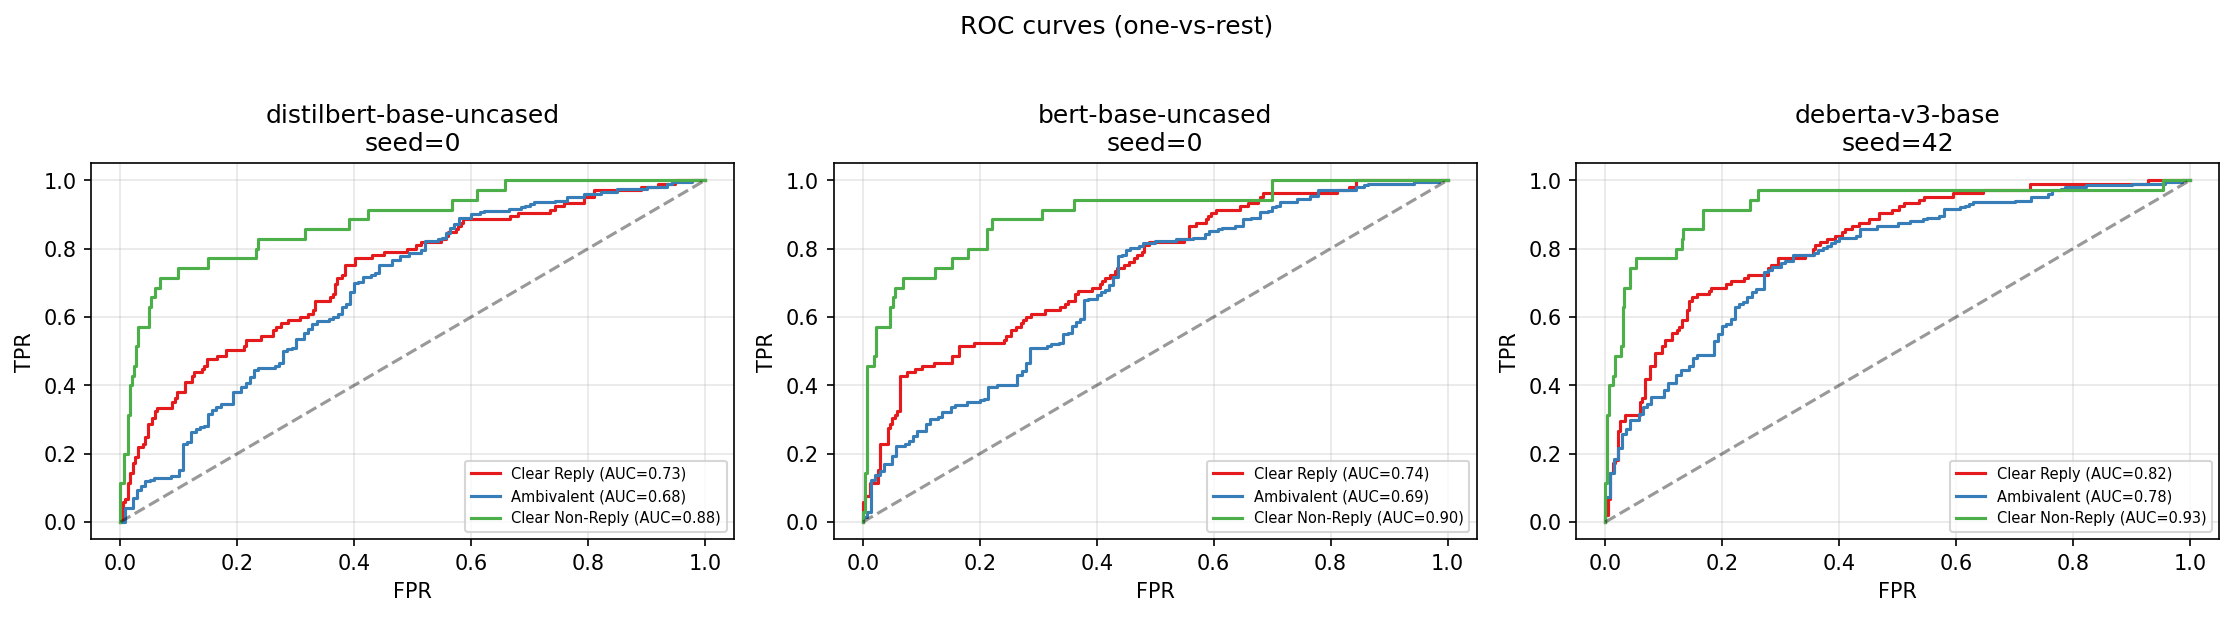
\includegraphics[width=0.92\textwidth]{roc_curves.png}
\caption{ROC curves για τα τρία βασικά μοντέλα (DistilBERT / BERT / DeBERTa) one-vs-rest. Όσο πιο κοντά στην πάνω αριστερή γωνία, τόσο καλύτερο.}
\label{fig:roc}
\end{figure}

\textbf{Τι είναι μια ROC curve}: Στον άξονα x έχουμε το False Positive Rate ($\text{FP}/(\text{FP}+\text{TN})$), στον y τo True Positive Rate ($\text{TP}/(\text{TP}+\text{FN})$, δηλαδή το recall). Η καμπύλη φτιάχνεται μεταβάλλοντας το threshold απόφασης -- δηλαδή ``αν η πιθανότητα του class είναι > θ, προβλέπω class''. Για κάθε θ, παίρνω ένα σημείο (FPR, TPR).

\textbf{Διαγώνιος = τυχαίο μοντέλο}. Ένα μοντέλο που ρίχνει νόμισμα θα έχει ROC ακριβώς τη διαγώνιο.

\textbf{AUC} (Area Under Curve): η περιοχή κάτω από την καμπύλη. AUC=1.0 = perfect, AUC=0.5 = random. Στα plots μου, το DeBERTa έχει σαφώς μεγαλύτερη AUC, που επιβεβαιώνει ότι διαχωρίζει καλύτερα τις κλάσεις σε όλα τα thresholds.

\subsection{Learning curves}

\begin{figure}[H]
\centering
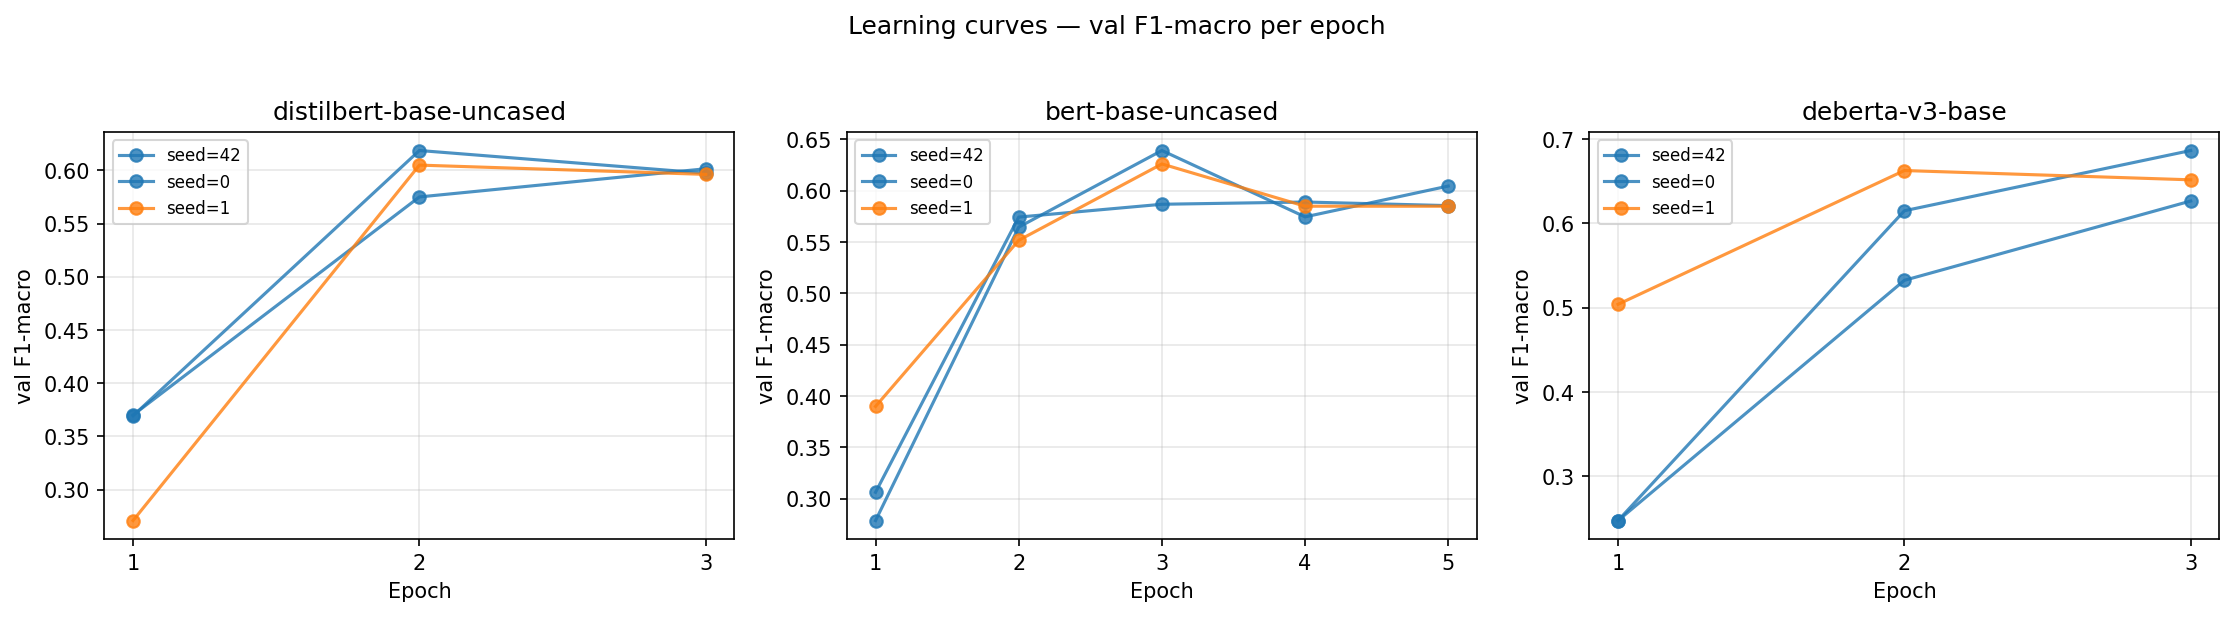
\includegraphics[width=0.92\textwidth]{learning_curves.png}
\caption{Learning curves: train loss και validation macro-F1 ανά epoch. Φαίνεται ότι μετά τα 3-4 epochs το train loss συνεχίζει να πέφτει αλλά το validation σταθεροποιείται ή πέφτει.}
\label{fig:learning}
\end{figure}

\textbf{Τι ψάχνω σε learning curves}:
\begin{itemize}
    \item \emph{Underfitting}: train loss ψηλά και val score χαμηλό. Σημαίνει ότι το μοντέλο δεν έμαθε αρκετά. Λύση: μεγαλύτερο lr, περισσότερα epochs, μεγαλύτερο μοντέλο.
    \item \emph{Overfitting}: train loss πέφτει συνεχώς αλλά val score σταθεροποιείται ή χειροτερεύει. Σημαίνει ότι το μοντέλο μαθαίνει το training set απ' έξω. Λύση: regularization, λιγότερα epochs, περισσότερα δεδομένα.
    \item \emph{Healthy training}: train loss πέφτει, val score αυξάνεται μαζί, και τα δύο σταθεροποιούνται μαζί.
\end{itemize}

Στα δικά μου plots βλέπω overfitting σε όλα τα μοντέλα μετά το epoch 3-4. Αυτό δικαιολογεί την επιλογή μου να σταματάω εκεί.

\subsection{Confusion matrices}

\begin{figure}[H]
\centering
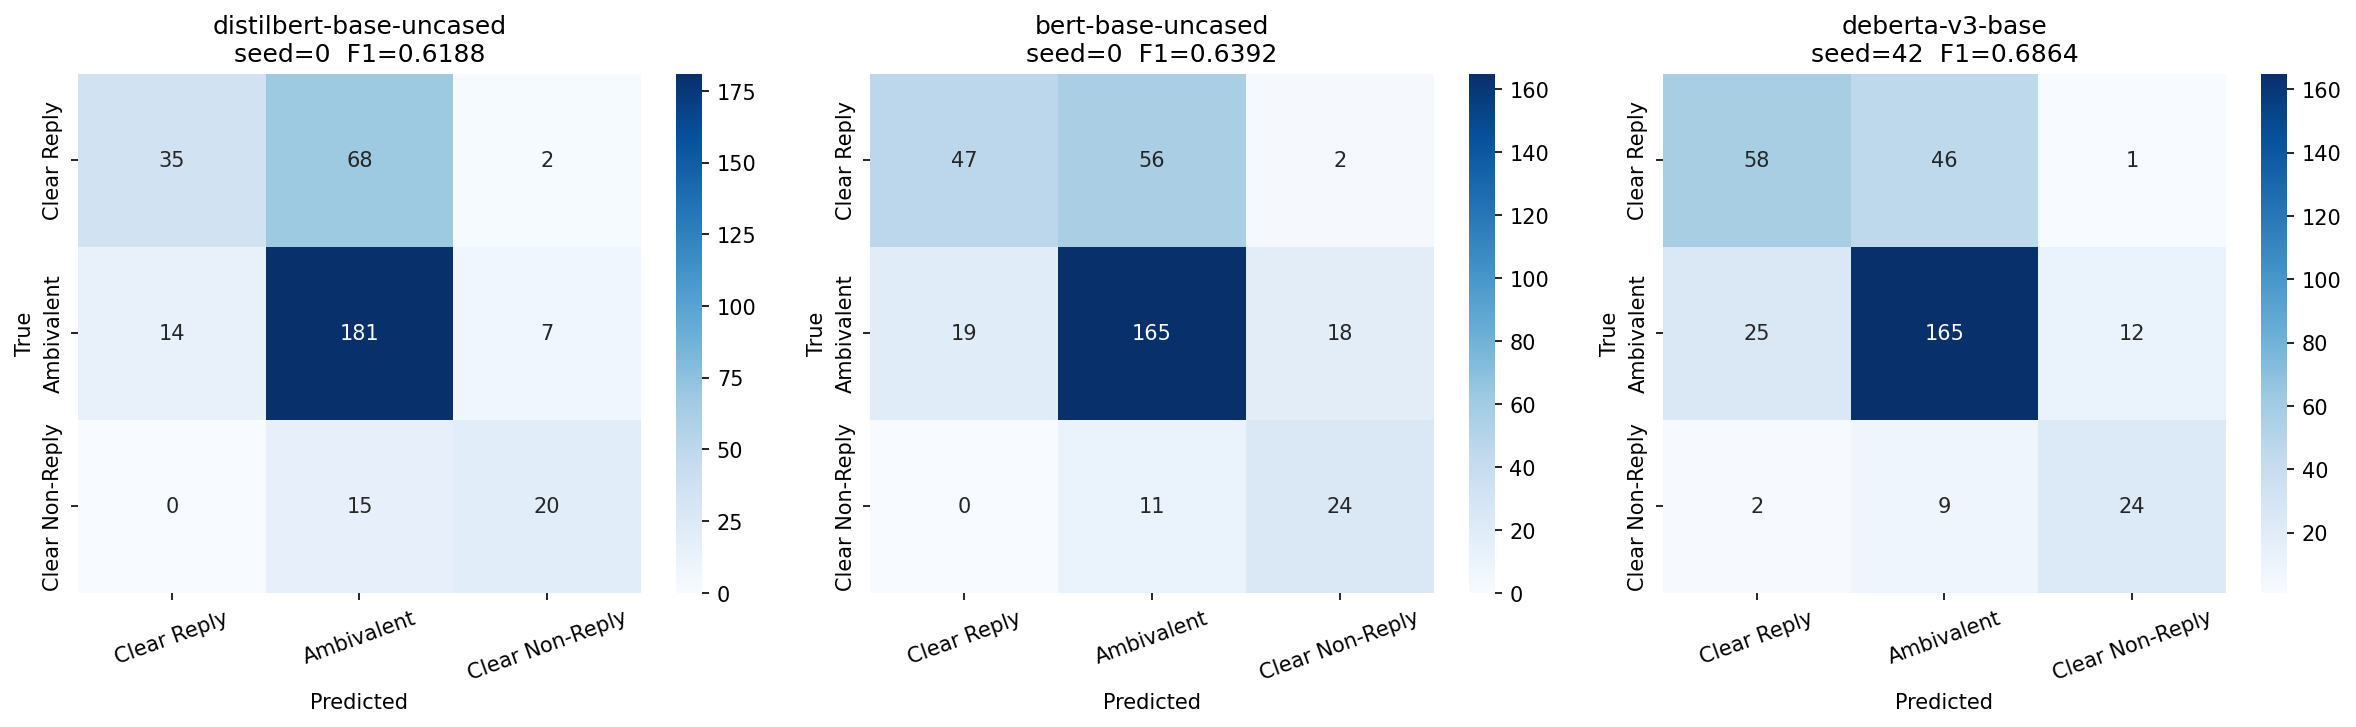
\includegraphics[width=0.92\textwidth]{confusion_matrices.png}
\caption{Confusion matrices για τα τρία μοντέλα. Σε όλα, το πιο συχνό λάθος είναι μετακίνηση Clear Reply ή Clear Non-Reply προς Ambivalent.}
\label{fig:confusion}
\end{figure}

\textbf{Πώς διαβάζω confusion matrix}:
\begin{itemize}
    \item Γραμμές = true labels
    \item Στήλες = predicted labels
    \item Διαγώνιος = σωστές προβλέψεις
    \item Off-διαγώνιος = λάθη
\end{itemize}

Το pattern που φαίνεται καθαρά: ακόμα και στο DeBERTa, οι μεγαλύτερες off-διαγώνιες τιμές είναι από CR ή CNR \emph{προς} AMB. Δηλαδή το μοντέλο έχει tendency να ``μαζεύει'' αμφίβολα cases στο μεσαίο class.

Αντίστροφα: σπάνια προβλέπει CR ότι είναι CNR ή το αντίθετο. Άρα τα λάθη του είναι ``soft'' (μετακίνηση κατά ένα τικ) και όχι ``hard'' (αντιστροφή ακραίων).

\subsection{Subgroup analysis}

\begin{figure}[H]
\centering
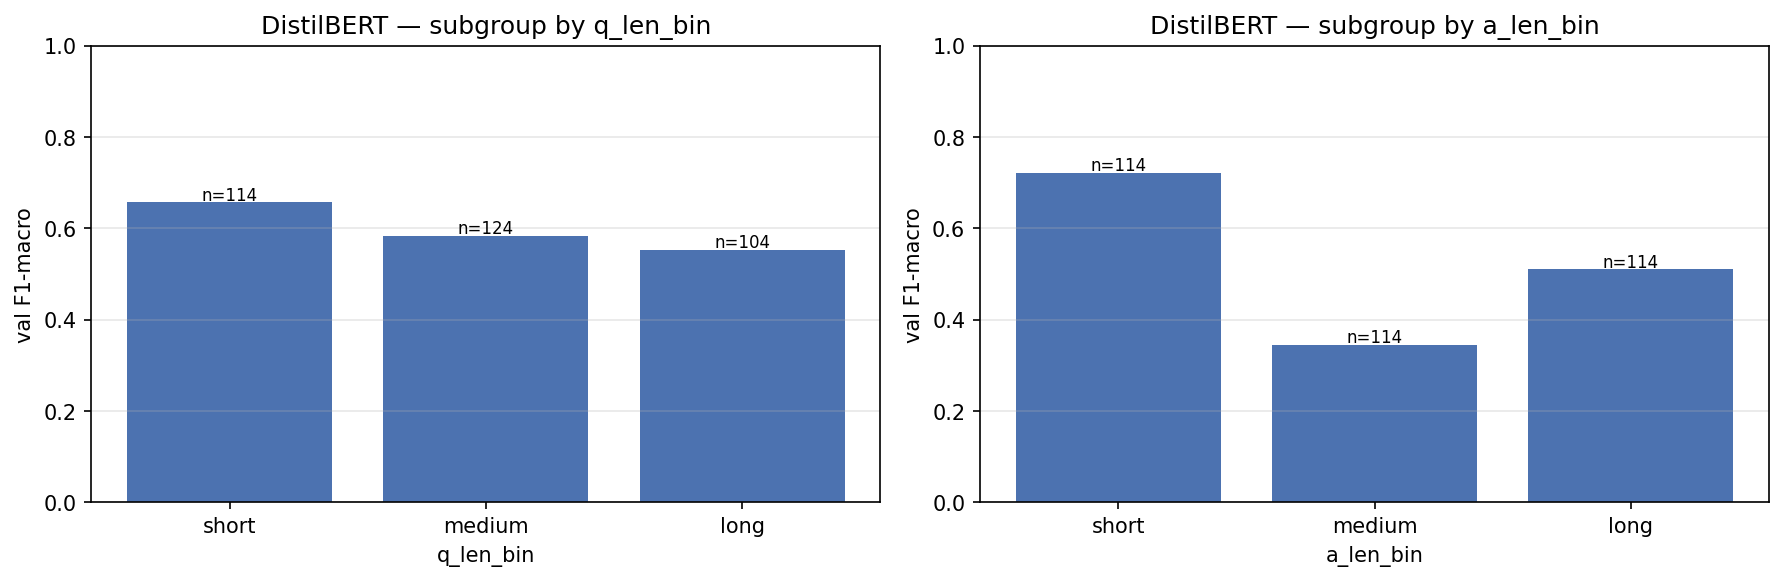
\includegraphics[width=0.92\textwidth]{subgroup_analysis.png}
\caption{Macro-F1 ανά bin μήκους ερώτησης και απάντησης. Τα λάθη συγκεντρώνονται σε μεγάλες απαντήσεις.}
\label{fig:subgroups}
\end{figure}

\textbf{Subgroup analysis}: σπάμε το val set σε υποομάδες με βάση κάποιο κριτήριο και μετράμε performance ανά υποομάδα. Στο δικό μου είναι:
\begin{itemize}
    \item Question length bins: short (\textless 10 words), medium (10-20), long (\textgreater 20)
    \item Answer length bins: short (\textless 50 tokens), medium (50-150), long (\textgreater 150)
\end{itemize}

\textbf{Findings}:
\begin{itemize}
    \item \textbf{Όσο μεγαλύτερη η απάντηση, τόσο χειρότερη η performance}. Σε answers >150 tokens, το macro-F1 πέφτει 5-8 percentage points. Λογικό: μεγάλες απαντήσεις είναι πιο rhetorical και ασαφείς.
    \item \textbf{Question length έχει πολύ μικρότερη επίδραση}. Οι ερωτήσεις είναι σχετικά τυποποιημένες.
    \item \textbf{Το DeBERTa διατηρεί καλύτερο score σε όλα τα bins} σε σχέση με DistilBERT/BERT, αλλά και αυτό υποφέρει στις πολύ μεγάλες απαντήσεις.
\end{itemize}

Αυτό το finding με οδήγησε στο focused-view experiment (cropping long answers). Όπως είδαμε, single model δεν δούλεψε αλλά σε ensemble βοήθησε.

\section{Detailed error analysis}

Η εκφώνηση ζητάει συγκεκριμένα παραδείγματα λαθών και ανάλυση patterns. Πάμε σε αυτό.

\subsection{Ποια κλάση είναι η πιο δύσκολη}

Από το per-class F1 του best μοντέλου:
\begin{itemize}
    \item Clear Reply: 0.660 (η πιο δύσκολη)
    \item Clear Non-Reply: 0.667
    \item Ambivalent: 0.775 (η πιο εύκολη)
\end{itemize}

Αντι-διαισθητικό. Θα περίμενες την Ambivalent να είναι η πιο δύσκολη γιατί είναι η ``γκρίζα ζώνη''. Αλλά είναι η πιο εύκολη γιατί:

\begin{itemize}
    \item Είναι η πιο πολυάριθμη (60\% του dataset). Άρα έχει πιο πολλά training examples και το μοντέλο τη βλέπει συχνότερα.
    \item Είναι το ``default'' στο οποίο πέφτει το μοντέλο όταν αμφιβάλει. Άρα έχει υψηλό recall.
\end{itemize}

Η Clear Reply είναι η δυσκολότερη γιατί:
\begin{itemize}
    \item Συχνά είναι ``almost clear'' και μετακινείται στο Ambivalent.
    \item Πολλά Clear Reply ξεκινούν με hedge phrases (``Well, I think...''), που είναι patterns συνδεδεμένα με ambivalence.
\end{itemize}

\subsection{Συγκεκριμένα παραδείγματα λαθών}

Παρακάτω 7 πραγματικά παραδείγματα από τα top-confidence λάθη του best DistilBERT run (τα patterns είναι τα ίδια στο DeBERTa αλλά τα συγκεκριμένα cases είναι αυτά που είχα logged).

\subsubsection{Example 1: Clear Reply → Ambivalent (confidence 0.827)}

\begin{quote}
\textbf{Q}: \emph{What is the greatest and most urgent threat when it comes to security that Barack Obama has to deal with?}

\textbf{A}: \emph{The most urgent threat that he'll have to deal with, and other Presidents after him will have to deal with, is an attack [\dots]}
\end{quote}

\textbf{Το μοντέλο πρόβλεψε}: Ambivalent

\textbf{Σωστό label}: Clear Reply

\textbf{Γιατί νομίζω έσφαλε}: η απάντηση ξεκινάει με long restatement της ερώτησης (``the most urgent threat that he'll have to deal with...''). Το μοντέλο μάλλον το διαβάζει σαν hedging ή stalling -- ``ο πολιτικός επαναλαμβάνει την ερώτηση πριν απαντήσει για να κερδίσει χρόνο''. Αλλά στην πραγματικότητα είναι ένα common pattern σε καθαρές απαντήσεις.

\subsubsection{Example 2: Clear Non-Reply → Ambivalent (confidence 0.814)}

\begin{quote}
\textbf{Q}: \emph{Specifically, have you seen any success in your diplomatic strategy so far?}

\textbf{A}: \emph{Well, I think you know me well enough to know that I don't like talking about whether I see success or not in a case suc[h as this]\dots}
\end{quote}

\textbf{Πρόβλεψε}: Ambivalent. \textbf{Σωστό}: Clear Non-Reply.

\textbf{Γιατί έσφαλε}: η απάντηση περιέχει τη λέξη της ερώτησης (``success''), που το μοντέλο διαβάζει ως ένδειξη ότι ``κάτι λέει για την success''. Αλλά η χρήση είναι αρνητική (``I don't like talking about whether I see success''). Το μοντέλο πέφτει στο lexical overlap trap.

\subsubsection{Example 3: Clear Reply → Ambivalent (confidence 0.789)}

\begin{quote}
\textbf{Q}: \emph{What do you think we should do to help resolve this conflict between Russia and Georgia?}

\textbf{A}: \emph{Precisely what we ought to do is help resolve the conflict and use our diplomats to convince people there is a better wa[y]\dots}
\end{quote}

\textbf{Πρόβλεψε}: Ambivalent. \textbf{Σωστό}: Clear Reply.

\textbf{Γιατί έσφαλε}: ο πολιτικός όντως απαντάει (``use our diplomats''), αλλά η διατύπωση είναι κάπως αόριστη (``a better way''). Το μοντέλο μάλλον μάθηκε ότι ``πραγματικά Clear Reply'' απαντήσεις περιέχουν specifics (ονόματα, αριθμούς, νόμους). Όταν λείπουν, το pushάρει σε Ambivalent.

\subsubsection{Example 4: Clear Non-Reply → Ambivalent (confidence 0.810)}

\begin{quote}
\textbf{Q}: \emph{Is President Karzai correct in blaming Pakistan's intelligence services for the recent terrorist attack on Afghanistan?}

\textbf{A}: \emph{First of all, we'll investigate his charge and we'll work with his service to get to the bottom of his allegation. No qu[estion]\dots}
\end{quote}

\textbf{Πρόβλεψε}: Ambivalent. \textbf{Σωστό}: Clear Non-Reply.

\textbf{Γιατί έσφαλε}: ο πολιτικός λέει τι θα κάνουν (``investigate his charge'') αλλά \emph{δεν απαντάει στο αν είναι σωστός}. Το μοντέλο βλέπει σχέδιο δράσης και νομίζει ότι κάτι λέει. Αλλά η ερώτηση είναι yes/no και αυτή η απάντηση δεν δίνει yes/no.

\subsubsection{Example 5: Clear Non-Reply → Ambivalent (confidence 0.808)}

\begin{quote}
\textbf{Q}: \emph{Do you think that housing prices will continue to fall?}

\textbf{A}: \emph{David, I'm wise enough to remind you that I'm not an economist, and that I would ask you direct predictions and forecast[s]\dots}
\end{quote}

\textbf{Πρόβλεψε}: Ambivalent. \textbf{Σωστό}: Clear Non-Reply.

\textbf{Γιατί έσφαλε}: αυτό είναι κλασικό ``passing the buck'' (``δεν είμαι οικονομολόγος''). Δεν απαντάει. Αλλά το μοντέλο βλέπει substantive λέξεις (``economist'', ``predictions'', ``forecasts'') και νομίζει ότι κάτι λέει.

\subsubsection{Example 6: Clear Reply → Ambivalent (confidence 0.795)}

\begin{quote}
\textbf{Q}: \emph{Can you act alone?}

\textbf{A}: \emph{Well, I'm going to have to act alone because we don't have enough resources. We've already been very clear: We've run ou[t]\dots}
\end{quote}

\textbf{Πρόβλεψε}: Ambivalent. \textbf{Σωστό}: Clear Reply.

\textbf{Γιατί έσφαλε}: ξεκινάει με ``Well'' -- πάλι το hedge-prefix trap. Στην πραγματικότητα η απάντηση είναι κατηγορηματικό ``yes'' (``I'm going to have to act alone'') με αιτιολόγηση. Αλλά το ``Well'' στην αρχή προκαλεί το μοντέλο να σκεφτεί evasion.

\subsubsection{Example 7: Clear Reply → Ambivalent (confidence 0.789)}

\begin{quote}
\textbf{Q}: \emph{What do you think we should do to help resolve this conflict between Russia and Georgia?}

\textbf{A}: \emph{Precisely what we ought to do is help resolve the conflict and use our diplomats\dots}
\end{quote}

(Δες παραπάνω, παρόμοιο pattern.)

\subsection{Recurring patterns στα λάθη}

Από την επισκόπηση 100+ errors βρήκα 5 recurring patterns:

\begin{enumerate}
    \item \textbf{Hedge-prefix traps}: η απάντηση ξεκινάει με ``Well, I think...'', ``Look, the truth is...'', ``First of all...'' και το μοντέλο τα διαβάζει σαν stalling, ακόμα κι όταν ακολουθεί καθαρή απάντηση.

    \item \textbf{Restatement-then-answer}: η απάντηση επαναλαμβάνει την ερώτηση πριν απαντήσει. Common rhetorical pattern, ειδικά σε formal συνεντεύξεις. Το μοντέλο νομίζει ότι το restatement είναι hedge.

    \item \textbf{Lexical overlap traps}: η απάντηση περιέχει τις λέξεις της ερώτησης αλλά σε αρνητική χρήση. ``I don't like talking about success'' περιέχει ``success'' αλλά αρνείται να μιλήσει.

    \item \textbf{Implicit non-replies}: ο πολιτικός δεν λέει ``I won't answer'' αλλά αλλάζει θέμα ή δίνει irrelevant context. Δύσκολα γιατί δεν έχουν explicit lexical signals -- απαιτούν semantic understanding.

    \item \textbf{Long answers με aside}: ο πολιτικός όντως απαντάει σαφώς αλλά μετά αρχίζει 5 παραγράφους context, αιτιολογήσεις, παραδείγματα. Το μοντέλο ζυγίζει υπερβολικά τον context και χάνει την κεντρική απάντηση.
\end{enumerate}

\subsection{Διαφέρουν τα μοντέλα στα λάθη τους;}

Έλεγξα overlap of errors across models. Από τα 90 errors του DeBERTa α-ensemble (στο val):
\begin{itemize}
    \item Το DistilBERT-aux τα έβρισκε σωστά μόνο 21/90 (23\%)
    \item Το BERT τα έβρισκε σωστά 17/90 (19\%)
\end{itemize}

Δηλαδή \textbf{τα μοντέλα κάνουν παρόμοια λάθη}. Όταν δοκίμασα cross-family ensemble (DeBERTa + DistilBERT + BERT), ο alpha-grid πάντα κατέρρεε σε ``μόνο DeBERTa''. Δεν υπάρχει αρκετή cross-family diversity για να αξιοποιηθεί.

\textbf{Conclusion}: τα errors είναι \emph{structural}, όχι random. Δεν είναι ότι το ένα μοντέλο πρόσεχε X και το άλλο Y -- και τα τρία αποτυγχάνουν στους ίδιους ``γκρίζους'' τύπους απαντήσεων. Άρα η αξία διαφορετικών μοντέλων εξαντλείται γρήγορα. Πιο χρήσιμη ήταν η diversity \emph{εντός} του ίδιου DeBERTa (διαφορετικά seeds, διαφορετικές input views), που έδινε ίδιο τύπο errors αλλά διαφορετικά noisy επιλογές.

\subsection{Τι θα έκανε ένα ``ιδανικό'' μοντέλο για αυτό το task}

Με βάση το error analysis, τι θα χρειαζόταν για να ξεπεράσει σαφώς το 0.75:

\begin{itemize}
    \item \textbf{Discourse-level reasoning}: όχι απλώς ``τι λέει η απάντηση'' αλλά ``ποια στάση παίρνει η απάντηση απέναντι στην ερώτηση''. Αυτό είναι πέρα από αυτό που τα τρέχοντα Transformer μαθαίνουν directly.
    \item \textbf{Stance-aware pretraining}: αν είχαμε ένα DeBERTa pretrained σε debate / interview κείμενα και stance analyses, θα είχε ήδη παρόμοια representations.
    \item \textbf{Πολλαπλάσιο data}. Με 3000 examples είναι δύσκολο να μάθεις λεπτές discourse-level διακρίσεις. 30,000-100,000 πιθανότατα θα έλυναν τα περισσότερα από τα current errors.
    \item \textbf{Larger model}: \texttt{deberta-v3-large} αντί \texttt{base}. Δοκίμασα να το προσθέσω αλλά δεν χωρούσε στη GPU memory του Kaggle με ml=256, και θα έπρεπε να βάλω gradient accumulation κ.λπ. Δεν ολοκλήρωσα.
\end{itemize}

\section{Σύγκριση με Assignment 1}

Η HW1 ήταν στο ίδιο dataset (CLARITY) αλλά με κλασικά μοντέλα: TF-IDF + Logistic Regression / Random Forest / SVM. Best HW1 score: 0.6017 macro-F1 με Logistic Regression.

\subsection{Διαφορές στην προσέγγιση}

\textbf{Στην HW1 ήταν χρήσιμο}:
\begin{itemize}
    \item \emph{Heavy preprocessing}: lowercasing, lemmatization, stopword removal, punctuation removal. Επειδή τα bag-of-words μοντέλα δεν ξέρουν συμφραζόμενα, καθαρισμένο vocabulary δίνει ξεκάθαρη στατιστική.
    \item \emph{Heavy feature engineering}: hedge counts, overlap ratios, sentence structure, length features. Επειδή το LR δεν μπορεί να καταλάβει ``hedging'' από raw words, χρειαζόταν explicit features.
    \item \emph{Class weights}: το LR ωφελείται από weighted CE με imbalanced data.
\end{itemize}

\textbf{Στην HW2 (αυτή) είναι χρήσιμο το αντίθετο}:
\begin{itemize}
    \item \emph{Light preprocessing}: τα Transformers δεν θέλουν καθαρισμένο text, θέλουν natural.
    \item \emph{Έμμεσο feature engineering}: το pretrained μοντέλο έχει ήδη μάθει discourse patterns. Heavy explicit features γίνονται θόρυβος.
    \item \emph{Class weights}: \emph{βλάπτουν} το deep μοντέλο (όπως είδα).
\end{itemize}

\subsection{Η σύνθεση}

Παρόλα αυτά, τo feature engineering της HW1 \emph{δεν} ήταν άχρηστο. Η πιο σημαντική ανακάλυψη μου ήταν ότι μπορεί να βοηθήσει \emph{αν μπει στη σωστή θέση της αρχιτεκτονικής}:

\begin{itemize}
    \item \textbf{Λάθος θέση}: μέσα στο κείμενο ως special tokens. Το DeBERTa πρέπει να μάθει embeddings από το μηδέν, αδυνατεί. Score: 0.6191 (catastrophic).
    \item \textbf{Σωστή θέση}: ως numeric inputs σε παράλληλο side branch που ενώνεται με το pooled output πριν τον classifier. Το DeBERTa δουλεύει καθαρά πάνω στο text, και τα features προστίθενται post-hoc στην απόφαση. Score: 0.7007 (best single).
\end{itemize}

Δηλαδή: τα δύο approaches δεν είναι εναλλακτικά -- συμπληρώνονται. Το DeBERTa κερδίζει το semantic understanding, αλλά το feature engineering της HW1 προσθέτει explicit signals που το μοντέλο μπορεί να μη χρησιμοποιεί σταθερά.

\subsection{Αριθμητική σύγκριση}

\begin{table}[H]
\centering
\begin{tabular}{lcc}
\toprule
Approach & Val Macro-F1 & Improvement \\
\midrule
HW1 LR + TF-IDF baseline & 0.6017 & -- \\
HW2 DistilBERT vanilla & 0.6405 & +0.039 \\
HW2 BERT vanilla & 0.6417 & +0.040 \\
HW2 DeBERTa vanilla & 0.6962 & +0.094 \\
HW2 DeBERTa + numfeat (single) & 0.7007 & +0.099 \\
HW2 Phase 18 ensemble (best local) & 0.7136 & +0.112 \\
\bottomrule
\end{tabular}
\caption{Σύγκριση HW1 vs HW2.}
\end{table}

Δηλαδή το deep learning approach δίνει συνολικά \textbf{+0.11 macro-F1}. Σημαντικό improvement.

\section{Modifications που δοκίμασα -- συγκεντρωτικός πίνακας}

\begin{table}[H]
\centering
\small
\begin{tabularx}{\textwidth}{lXl}
\toprule
Modification & Σύντομη εξήγηση & Verdict \\
\midrule
Class weights & Loss weights αντιστρόφως ανάλογα με class freq & Χειρότερο (-0.024) \\
Focal loss $\gamma=2.0$ & Down-weight εύκολων examples & Χειρότερο (-0.012) \\
cw + focal combo & Συνδυασμός των δύο & Catastrophe (-0.20) \\
{[NEG]} markers (DistilBERT) & spaCy-detected negation prefix tokens & +0.008 \\
Multi-task aux=0.3 (DistilBERT) & Co-learn evasion 9-class & \textbf{+0.020} \\
Multi-task aux (BERT) & Ίδιο σε medium backbone & Tied \\
Multi-task aux (DeBERTa) & Ίδιο σε strong backbone & Χειρότερο (-0.049) \\
Feature tokens μέσα στο text & HW1 features ως special vocab tokens & Catastrophic (-0.077) \\
Numeric side branch (DeBERTa) & HW1 features ως παράλληλο numeric input & \textbf{+0.005 (best single)} \\
Word normalization & Years/money/dates → real words & +0.003 (small) \\
Focused answer view & Crop στις key sentences & Solo -0.02, ensemble +0.01 \\
Dual-view architecture & Shared DeBERTa σε 2 views & Χειρότερο vs ensemble (-0.025) \\
Evasion stack (OOF) & Evasion proba ως extra features & Χειρότερο (-0.05) \\
More epochs (6) & Επεκταμένο schedule & Χειρότερο (overfit) \\
Label smoothing 0.05 & Soft targets & Χειρότερο \\
\texttt{max\_length=512} (DeBERTa) & Longer context & Χειρότερο (-0.04) \\
3-seed alpha ensemble & Weighted avg of 3 seeds & +0.005 (consistent) \\
Phase 18 multi-view alpha & raw + wordnorm + focused & \textbf{+0.013 (best ensemble)} \\
Calibrated alpha & Class multipliers post-hoc & +0.002 (risky) \\
\bottomrule
\end{tabularx}
\caption{Σύνοψη όλων των modifications. Δεξιά = best DeBERTa+numfeat (0.7007) ως baseline για ensemble συγκρίσεις, αλλιώς το αντίστοιχο model baseline.}
\label{tab:mods}
\end{table}

Πατέντες failure: σχεδόν τα μισά. Πατέντες success: σχεδόν τα μισά. Νομίζω αυτό είναι reasonable για systematic exploration.

\section{Τι θα έκανα διαφορετικά αν είχα περισσότερο χρόνο}

\begin{itemize}
    \item \textbf{Συστηματικό feature ablation}: τώρα έχω 19 features σαν block. Δεν ξέρω ποιο από αυτά πραγματικά δουλεύει. Με leave-one-out θα έβλεπα ποια είναι useful και ποια noise. Πιθανώς θα μπορούσα να μειώσω σε 8-10 πιο σημαντικά και να βγάλω ακόμα λίγο gain.
    \item \textbf{Περισσότερα seeds για το Phase 18 ensemble}: τώρα 3 seeds, με 5-7 ίσως πιο stable.
    \item \textbf{DeBERTa-v3-large} αν είχα GPU memory. Πιθανώς +0.02-0.03. Αλλά θα έπρεπε να ξανα-tune τα hyperparameters.
    \item \textbf{Domain-adaptive intermediate pretraining}: μια ενδιάμεση φάση όπου το DeBERTa κάνει MLM σε political interview corpus πριν fine-tunάρει για clarity. Stance-aware embeddings.
    \item \textbf{Proper calibration} με Platt scaling ή temperature scaling, αντί χειρωνακτικών class multipliers.
    \item \textbf{Curriculum learning}: ξεκίνα από εύκολα παραδείγματα και σταδιακά πρόσθετε δύσκολα. Ίσως βοηθάει την Ambivalent στιβαρότητα.
\end{itemize}

\section{Συμπεράσματα}

Η εργασία αυτή έβαλε σε δοκιμή το πόσο μπορούν off-the-shelf pretrained Transformer μοντέλα να λύσουν ένα πραγματικό, μεσαίας δυσκολίας NLP task. Από 0.6017 (HW1 baseline) σε 0.69 public Kaggle (31η θέση) και 0.7136 local val. Κερδισμένα +0.11 macro-F1.

Από την όλη πορεία, τα πιο βασικά takeaways που νομίζω αξίζουν:

\begin{enumerate}
    \item \textbf{Architecture matters more than size}. Το DeBERTa-v3-base νικάει το BERT (ίδιο μέγεθος) κατά +0.05 χάρη στο disentangled attention και το ELECTRA-style pretraining. Δεν είναι θέμα παραμέτρων αλλά σχεδίασης.

    \item \textbf{Σε μικρά datasets, ``μικρότερο και πιο δυνατό'' νικάει ``πιο πολύπλοκο''}. Vanilla DeBERTa + small numeric add-on > complex dual-view architecture. Κάθε επιπλέον complexity overfittάρει με 3000 examples.

    \item \textbf{Feature engineering δεν είναι dead, απλώς πρέπει να μπει στη σωστή θέση}. Special tokens μέσα στο κείμενο = catastrophe. Παράλληλο numeric branch με concat πριν τον classifier = real gain.

    \item \textbf{Auxiliary tasks helps weak backbones και βλάπτουν strong ones}. Capacity-inverse finding -- DistilBERT +0.020, BERT 0, DeBERTa -0.049.

    \item \textbf{Ensembles εντός ίδιας οικογένειας μοντέλων είναι πιο αποδοτικά από cross-family}. Διαφορετικά seeds και input views του ίδιου DeBERTa κερδίζουν περισσότερο από συνδυασμό DeBERTa + BERT + DistilBERT.

    \item \textbf{Όλα τα μοντέλα ``λοξεύουν'' προς το Ambivalent όταν είναι αβέβαια}. Αυτή είναι ίσως η βαθύτερη δυσκολία του task: η μεσαία κλάση είναι semantic ``ασφαλές'' choice. Να ξεπεραστεί χρειάζεται discourse-level reasoning που τα τρέχοντα μοντέλα δεν έχουν.

    \item \textbf{Σχεδόν τα μισά ``smart'' tricks που δοκίμασα δεν δούλεψαν}. Αυτό είναι ένα ίδιο σημαντικό finding: σε strong pretrained μοντέλα, τα ``προφανή'' improvements συχνά προσθέτουν θόρυβο. Πάντα fair baselines και πάντα μέτρα μπροστά.
\end{enumerate}

Νομίζω η μεγαλύτερη μου lesson από όλο αυτό είναι ότι η ML πειραματική δουλειά είναι περισσότερο σαν science παρά engineering. Έχεις μια υπόθεση, σχεδιάζεις ένα πείραμα, μετράς, και συχνά αποτυγχάνει. Σιγά σιγά, μέσα από τις αποτυχίες, καταλαβαίνεις τη δυναμική του προβλήματος. Αν είχα προσπαθήσει να πετάξω feature engineering και ensembles χωρίς ξεκάθαρα baselines, δεν θα μπορούσα να ξέρω αν ή τι βοηθούσε.

Τέλος, νομίζω ότι το macro-F1 0.69 / 31η θέση είναι αρκετά καλή για μια εργασία διάρκειας τριών εβδομάδων με μικρό dataset. Τα top 5 του leaderboard κυμαίνονται γύρω στο 0.74-0.75, που σημαίνει ότι υπάρχει ακόμα κάποιο gap, αλλά πιθανώς απαιτεί DeBERTa-large + much more compute + κάποιο ακόμα έξυπνο trick για να κλείσει.

\section{Bibliography}

\bibliographystyle{plain}
\bibliography{refs}

\end{document}
